%!TEX program = xelatex
\documentclass[a4paper,12pt]{report}
\usepackage{indentfirst} 
\usepackage{ctex}
%\usepackage{xeCJK}
\usepackage{times}
\usepackage{graphicx,float}
\usepackage{subcaption}
\usepackage{setspace}
\usepackage{fancyhdr}
% \usepackage{graphicx}
\usepackage{wrapfig}
\usepackage{array}
\usepackage{fontspec,xunicode,xltxtra}
\usepackage{titlesec}
\usepackage{titletoc}
\usepackage[titletoc]{appendix}
\usepackage[top=30mm,bottom=30mm,left=20mm,right=20mm]{geometry}
\usepackage{cite}
\usepackage{listings}
\usepackage{float}
\usepackage[framed,numbered,autolinebreaks,useliterate]{mcode} % 插入代码
\usepackage{listings}

\lstset{
	%backgroundcolor=\color{red!50!green!50!blue!50},%代码块背景色为浅灰色
%	rulesepcolor= \color{gray}, %代码块边框颜色
	breaklines=true,  %代码过长则换行
	numbers=left, %行号在左侧显示
	numberstyle= \small,%行号字体
	%keywordstyle= \color{blue},%关键字颜色
	commentstyle=\color{gray}, %注释颜色
%	frame=shadowbox%用方框框住代码块
	frame=single,
	escapeinside=``    % 代码包含中文
}

\XeTeXlinebreaklocale "zh"
\XeTeXlinebreakskip = 0pt plus 1pt minus 0.1pt

%---------------------------------------------------------------------
%	页眉页脚设置
%---------------------------------------------------------------------
\fancypagestyle{plain}{
	\pagestyle{fancy}      %改变章节首页页眉
}

\pagestyle{fancy}
\lhead{\kaishu~``计算机网络''实验报告~}
\rhead{\kaishu~~实验4:基于套接字的网络程序设计}
\cfoot{\thepage}

%---------------------------------------------------------------------
%	章节标题设置
%---------------------------------------------------------------------
\titleformat{\chapter}{\centering\zihao{-1}\heiti}{实验\chinese{chapter}}{1em}{}
\titlespacing{\chapter}{0pt}{*0}{*6}

%---------------------------------------------------------------------
%	摘要标题设置
%---------------------------------------------------------------------
\renewcommand{\abstractname}{\zihao{-3} 摘\quad 要}

%---------------------------------------------------------------------
%	参考文献设置
%---------------------------------------------------------------------
\renewcommand{\bibname}{\zihao{2}{\hspace{\fill}参\hspace{0.5em}考\hspace{0.5em}文\hspace{0.5em}献\hspace{\fill}}}

%---------------------------------------------------------------------
%	引用文献设置为上标
%---------------------------------------------------------------------
\makeatletter
\def\@cite#1#2{\textsuperscript{[{#1\if@tempswa , #2\fi}]}}
\makeatother

%---------------------------------------------------------------------
%	目录页设置
%---------------------------------------------------------------------
\titlecontents{chapter}[0em]{\songti\zihao{-4}}{\thecontentslabel\ }{}
{\hspace{.5em}\titlerule*[4pt]{$\cdot$}\contentspage}
\titlecontents{section}[2em]{\vspace{0.1\baselineskip}\songti\zihao{-4}}{\thecontentslabel\ }{}
{\hspace{.5em}\titlerule*[4pt]{$\cdot$}\contentspage}
\titlecontents{subsection}[4em]{\vspace{0.1\baselineskip}\songti\zihao{-4}}{\thecontentslabel\ }{}
{\hspace{.5em}\titlerule*[4pt]{$\cdot$}\contentspage}

\renewcommand\thesection{\arabic{section}}
\renewcommand\thesubsection{\arabic{section}.\arabic{subsection}}
\setcounter{tocdepth}{3}
\setcounter{secnumdepth}{3}
\begin{document}
%---------------------------------------------------------------------
%	封面设置
%---------------------------------------------------------------------
\begin{titlepage}
	\begin{center}
		
    
\includegraphics[width=1.0\textwidth]{figure//nankai.jpg}\\
    % \vspace{10mm}
    % \textbf{\zihao{2}\kaishu{软件学院}}\\[0.8cm]
    \vspace{50mm}
    \textbf{\zihao{1}\heiti{ 《计算机网络》实验报告}}\\[1cm]
    \textbf{\zihao{2}\heiti{ (2022\textasciitilde2023学年第一学期)}}\\[1cm]
    % \textbf{\zihao{3}\heiti{ 实验1: Wireshark 软件使用与ARP 协议分析}}\\[2cm]
	\vspace{\fill}
	
\setlength{\extrarowheight}{2mm}
{\songti\zihao{3}	
\begin{tabular}{rl}

	{\makebox[4\ccwd][s]{实验名称:}}& ~\kaishu 基于套接字的网络程序设计\\
	{\makebox[4\ccwd][s]{学\qquad 院:}}& ~\kaishu 软件学院\\
		{\makebox[4\ccwd][s]{姓\qquad 名:}}& ~\kaishu 张怡桢\\

    {\makebox[4\ccwd][s]{学\qquad 号:}}& ~\kaishu 2013747 \\

	{\makebox[4\ccwd][s]{指导老师:}} & ~\kaishu 张圣林\\

\end{tabular}
 }\\[2cm]
\vspace{\fill}
\zihao{4}
%2021\textasciitilde 2022秋季学期\\
%使用\LaTeX 撰写于
    \today
	\end{center}	
\end{titlepage}


%---------------------------------------------------------------------
%  目录页
%---------------------------------------------------------------------
\tableofcontents % 生成目录

%---------------------------------------------------------------------
%  实验一
%---------------------------------------------------------------------
\chapter*{基于套接字的网络程序设计
}
\setcounter{page}{1}
\begin{spacing}{1.5}
\songti\zihao{-4}

%\section{分工情况}
 %\begin{itemize}
 %	\item 张三:
 %	\item 李四:
 %	\item 六六:
 %\end{itemize}
\section{套接字基础与 UDP 通信}
\subsection{实验目的}
熟悉基于 Python 进行 UDP 套接字编程的基础知识,掌握使用 UDP 套接字发送和接收数据包, 以及设置正确的套接字超时,了解 Ping 应用程序的基本概念,并理解其在简单判断网络状态,例如 计算数据包丢失率等统计数据方面的意义。
\subsection{实验内容}
1. 操作系统附带的标准 Ping 命令使用 ICMP 进行通信,本实验要求学生编程实现一个简单的, 非标准的,基于 UDP 进行通信的 Ping 程序。学生需要用 Python 编写一个 Ping 客户端。客户 端程序发送一个 ping 报文,然后接收一个从已经提供的服务器上返回的对应 pong 报文,并 计算出从该客户发送 ping 报文到接收到 pong 报文为止的往返时延(Round-Trip Time,RTT)。

2. 在客户端程序一次执行过程中,学生编写的的 Ping 客户端程序需经 UDP 向服务器发送 10 个 ping 报文。对于每个报文,当对应的 pong 报文返回时,客户端程序要确认并打印输出 RTT 值;在整个执行过程中,客户端程序需要考虑分组丢失情况,客户端最多等待 1 秒,超过该 时长则打印丢失报文。

\paragraph*{进阶任务}
修改代码,在程序运行结束时,计算所有 ping 消息的最 小、最大和平均 RTT,并计算丢包率(丢失数据包在总数据包中所占有的百分比)。即构造出一个符合标准 Windows 版 Ping 程序工作模式的基于 UDP 版 Ping 程序。

\subsection{实验原理}
UDP 作为一种传输层协议,只提供了无连接通信,且不对传送的数据包进行可靠性保证,因此 只适合于一次传输少量数据的应用场景,如果在传输过程中需要保证可靠性,则这种可靠性应该由 应用层负责。本实验创建的 Ping 程序正是一种不需要保证可靠性的程序,并需要利用这种不可靠性 来测量网络的联通情况。

虽然 UDP 不保证通信的可靠性,包到达的顺序,也不提供流量控制。但正是因为 UDP 的控制选 项较少,所以在数据传输过程中延迟小、数据传输效率高,一些对可靠性要求不高,但对性能等开销 更敏感的应用层协议会选择基于 UDP 进行实现,常见的使用 UDP 的应用层协议包括 TFTP、SNMP、 NFS、DNS、BOOTP 等,通常占用 53(DNS)、69(TFTP)、161(SNMP)等端口。

基于 UDP 的无连接客户/服务器在 Python 实现中的工作流程如下:

1. 首先在服务器端通过调用socket()创建套接字来启动一个服务器;

2. 服务器调用bind() 指定服务器的套接字地址,然后调用recvfrom()等待接收数据。

3. 在客户端调用socket()创建套接字,然后调用sendto()向服务器发送数据。

4. 服务器接收到客户端发来的数据后,调用sendto()向客户发送应答数据,

5. 客户调用recvfrom()接收服务器发来的应答数据。

6. 一旦数据传输结束,服务器和客户通过调用close()来关闭套接字。

注意在不同的计算机语言实现中,上述调用的名字和具体工作流程可能略有不同。基于 Python 的 UDP 程序工作详细流程如图\ref{1}所示。

\begin{figure}[H]
  \centering
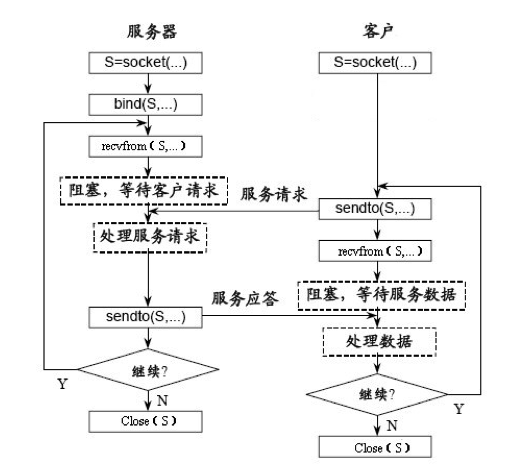
\includegraphics[width=10cm]{figure/1.png}
\caption{无连接客户/服务器流程图}
\label{1}
\end{figure}

基于 Python 进行 UDP 消息的接收操作时,Python 程序将工作在阻塞状态
,即未收到数据包时, Python 程序将挂起等待而不会继续执行。
如果程序运行中网络连接出现了问题,导致数据包无法及 时到达,这种阻塞式
的工作模式将会严重的干扰程序的执行。为了解决这个问题,Python 的套接字 
通信库提供了一种“超时”机制来防止程序卡死。在 Python 套接字程序中
,套接字对象提供了一个settimeout()方法来限制recvfrom()函数的等待时间,当recvfrom()函数阻塞等待超过这个时 间(一般称为“超时时间”)后仍然没有收到数据时,程序将会抛出一个异常来说明发生了等待数据 接收超时事件。在编写 Python 网络通信程序时,可以利用这个机制来判断是否接收数据超时。

\subsection{实验过程与截图(含进阶任务)}
基于图\ref{1}中的 UDP 的无连接客户/服务器在 Python 实现中的工作流程,实现的代码满足以下要求:

1. 使用 UDP 发送 ping 消息(注意:因为 UDP 是无连接协议,不需要建立连接。

2. 如果服务器在 1 秒内响应,则打印该响应消息;计算并打印每个数据包的往返时间 RTT(以 秒为单位);

3. 否则,打印“请求超时”(中英文皆可)。

UDPServer端代码如下:
\begin{spacing}{1}  
	\begin{lstlisting}[language={Python}]
    # lab1 服务端代码
    import random
    from socket import *
    
    # 创建一个UDP套接字(SOCK_DGRAM)
    serverSocket = socket(AF_INET, SOCK_DGRAM)
    # 绑定IP地址和端口号
    Host = ''
    serverSocket.bind((Host, 9999))
    
    while True:
        print('==================2013747zyz==================')
        print('UDP Server is starting...')
        # 返回参数1和参数2之间的任意整数, 闭区间
        rand = random.randint(0, 10)
        # 服务端调用recvfrom()等待接收数据,此时阻塞
        message, address = serverSocket.recvfrom(1024)
        response = 'Wrong!'
        print("UDP Client {} makes a Ping request\n".format(address))
        if message == 'Ping'.encode("utf-8"):
            response = 'Pong'
        if rand < 4:  # 模拟丢失30%的客户端数据包
            print('Data lost')
            continue
        print('success')
        # 服务器接收到客户端发来的数据后,调用sendto()向客户发送应答数据
        serverSocket.sendto(response.encode("utf-8"), address)
    
    serverSocket.close()
    
		\end{lstlisting}
\end{spacing}

UDPClient端代码如下:
\begin{spacing}{1}  
	\begin{lstlisting}[language={Python}]
    # lab1 用户端代码
    from socket import *
    import time
    
    serverHost = '114.116.206.13'  # 服务器地址 根据服务器地址进行修改即可
    serverPort = 9999  # 服务器建立连接的端口号
    
    clientSocket = socket(AF_INET, SOCK_DGRAM)  # 创建socket套接字
    clientSocket.settimeout(1)  # 为socket设置时延为1秒
    
    timeList = []  # 存放RTT
    totalReq = 10  # 发送的报文总数
    loseReq = 0  # 记录丢包数
    
    print('UDP Client makes a Ping request to Server[%s:%d]  :' % (serverHost, serverPort))
    for i in range(0, totalReq):
        start = time.perf_counter()  # RRT开始计数时间
        try:
            # 向服务器发送‘Ping’服务请求,将信息转换为byte后发送到指定服务器端
            clientSocket.sendto('Ping'.encode("utf-8"), (serverHost, serverPort))
    
            # 调用recvfrom()函数接收服务器发来的应答数据
            recvData, address = clientSocket.recvfrom(1024)
            # 超时处理,等到时间超过1秒,捕获抛出的异常后打印丢失报文,进行下一步操作
            RTT = (time.perf_counter() - start) * 1000
            # 存放RTT
            timeList.append(RTT)
            # 若服务器响应正常,收到‘Pong’
            if recvData.decode() == 'Pong':
                print('Num: %d reply from %s : time = %.5fms' % (i + 1, serverHost, RTT))
            else:
                print(recvData)
        # 若请求超时
        except Exception as e:
            loseReq += 1
            print('Num: %d out of time' % (i + 1))
    # 关闭套接字
    clientSocket.close()
    
    print()
    print('The Ping Message of %s :' % serverHost)
    print('   UDP: sent = %d,got = %d,loss = %d (%d%% packet loss rate)' % (i + 1, i - loseReq + 1, loseReq, (loseReq / (i + 1)) * 100))
    print("RTT_TIME(ms):")
    try:
        print("   min_RRT = %.5fsms,max_RRT = %.5fsms,average_RRT = %.5fsms" % (min(timeList), max(timeList), sum(timeList)/len(timeList)))
    except ValueError:
        print("   min_RRT = 0ms,max_RRT = 0ms,average_RRT = 0ms")
		\end{lstlisting}
\end{spacing}

在同一主机上先运行服务端,再运行客户端程序,客户端和服务端截图如图\ref{3},\ref{4},其中client ping server后得到的ping 消息的最小、最大和平均 RTT以及丢包率(丢失数据包在总数据包中所占有的百分比)都实现了,即构造出了一个符合标准 Windows 版 Ping 程序工作模式的基于 UDP 版 Ping 程序:
\begin{figure}[H]
  \centering
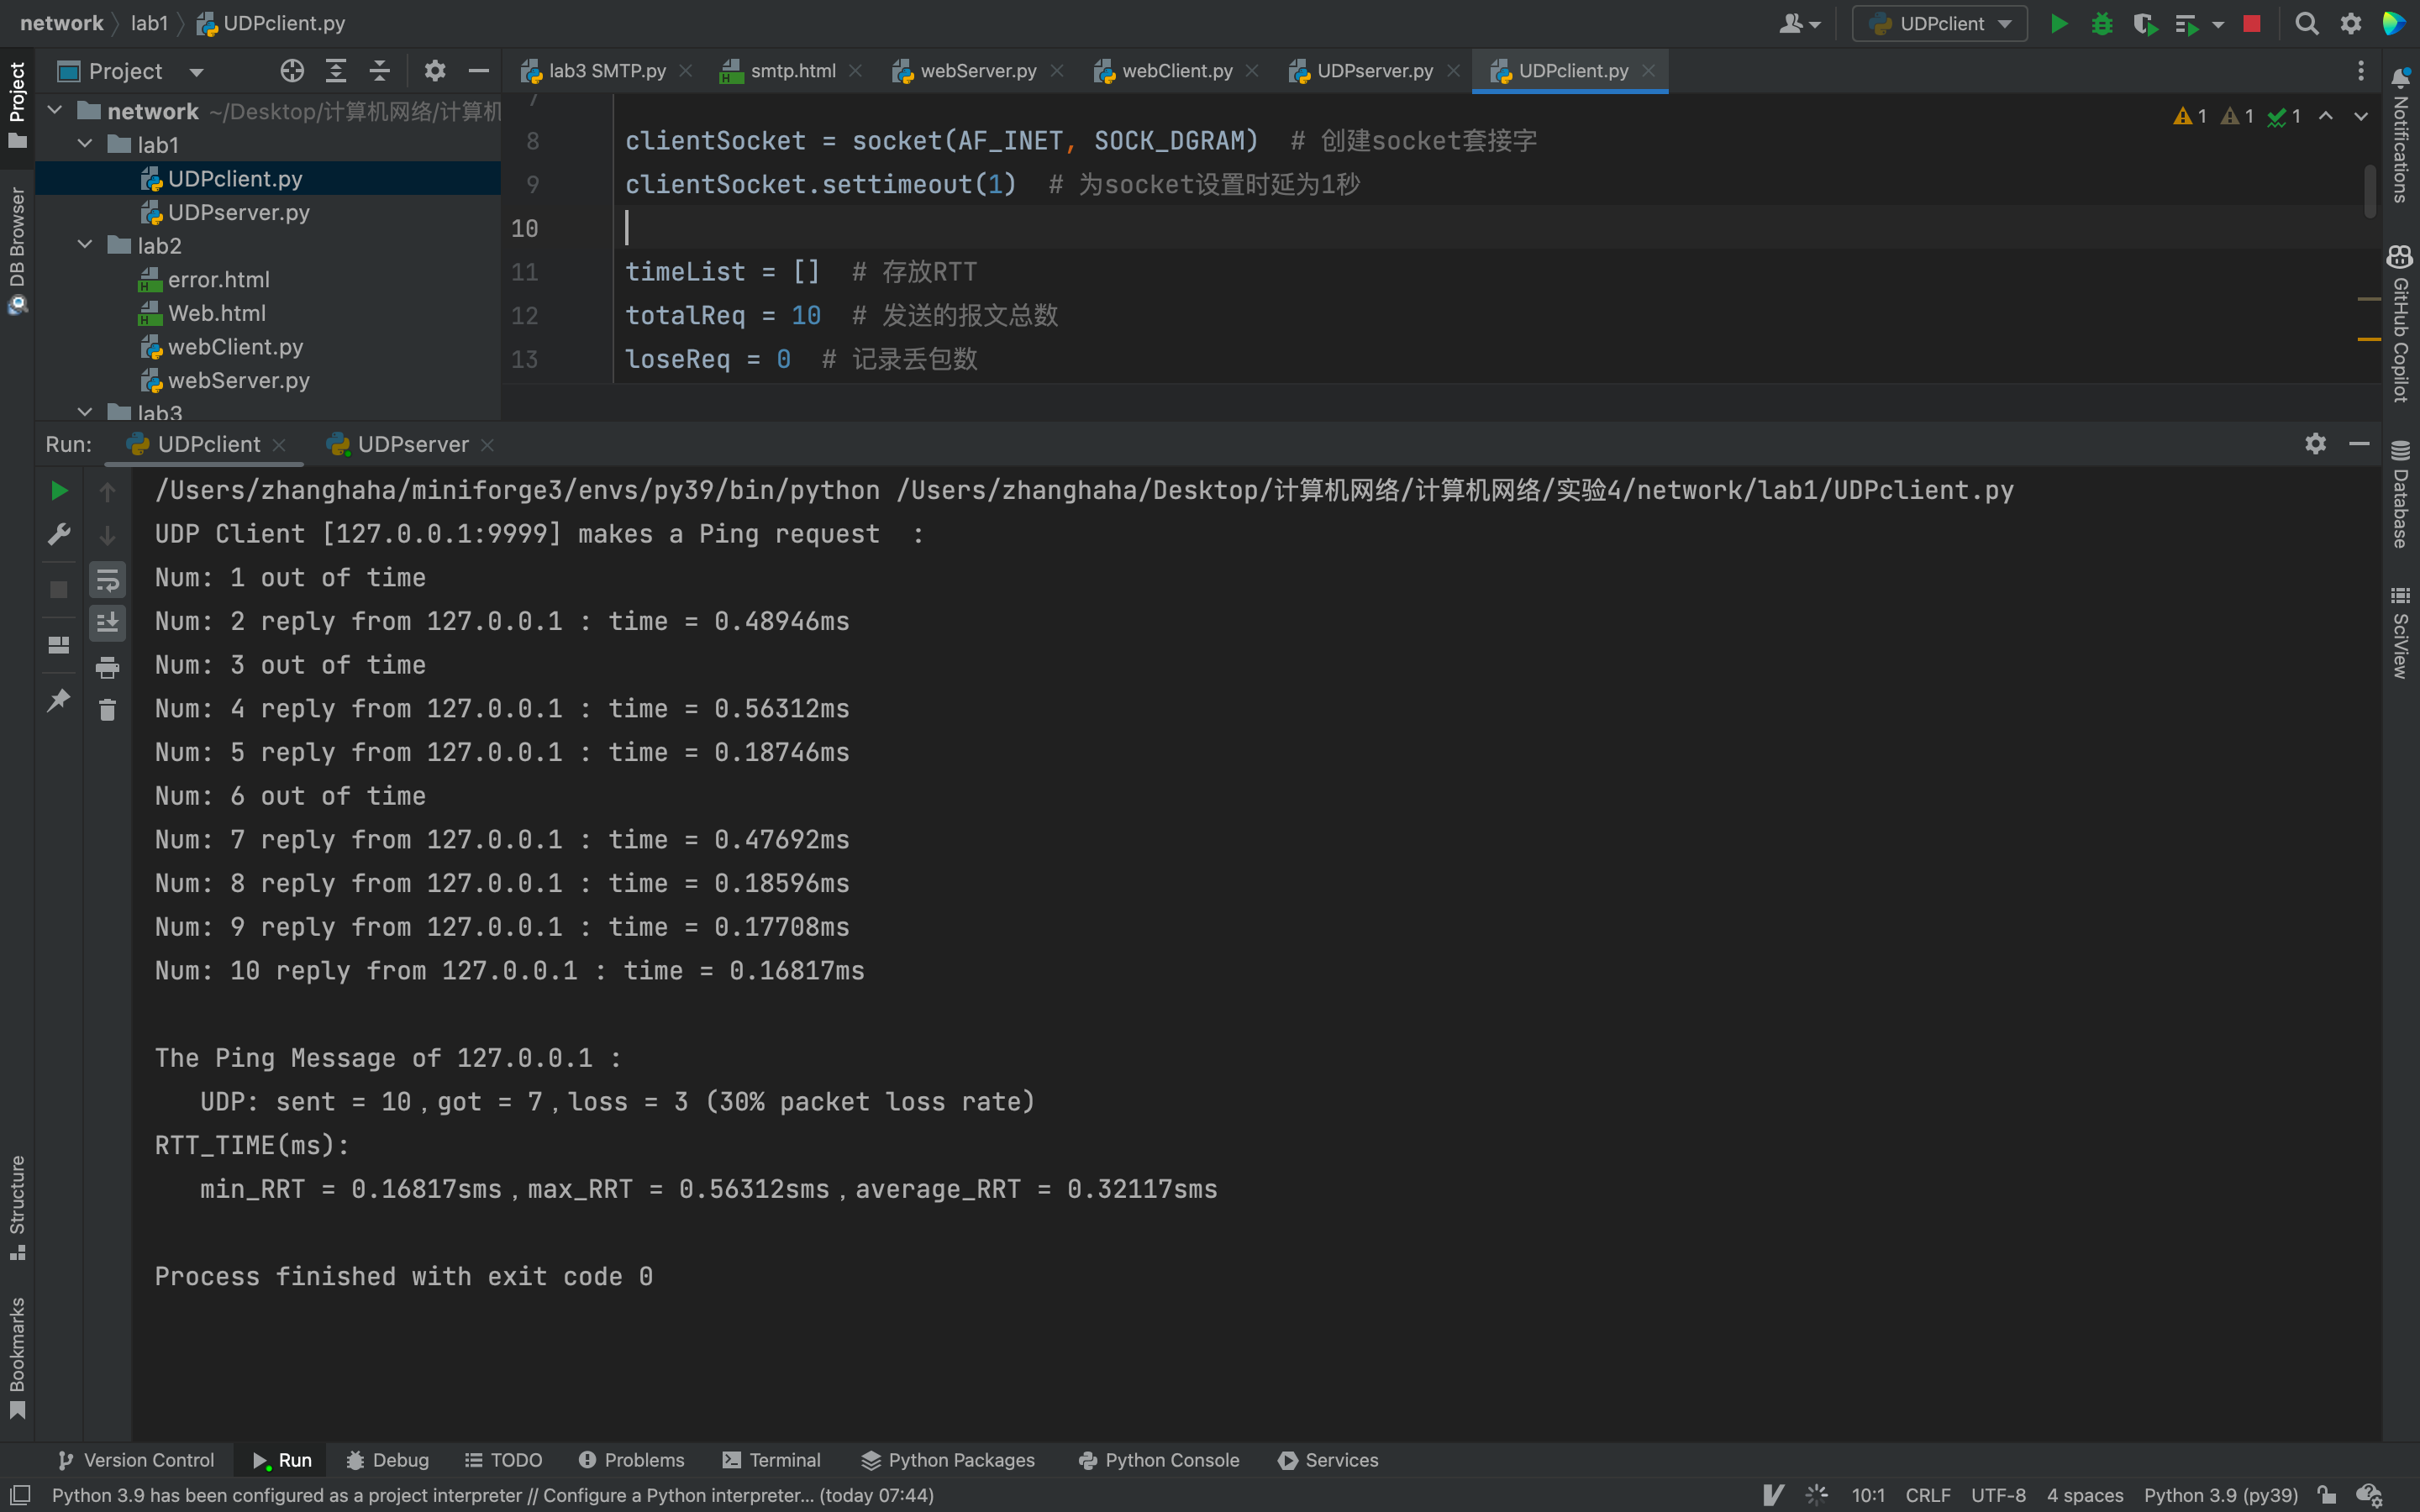
\includegraphics[width=10cm]{figure/udp_c_w.png}
\caption{UDP客户端}
\label{3}
\end{figure}
\begin{figure}[H]
  \centering
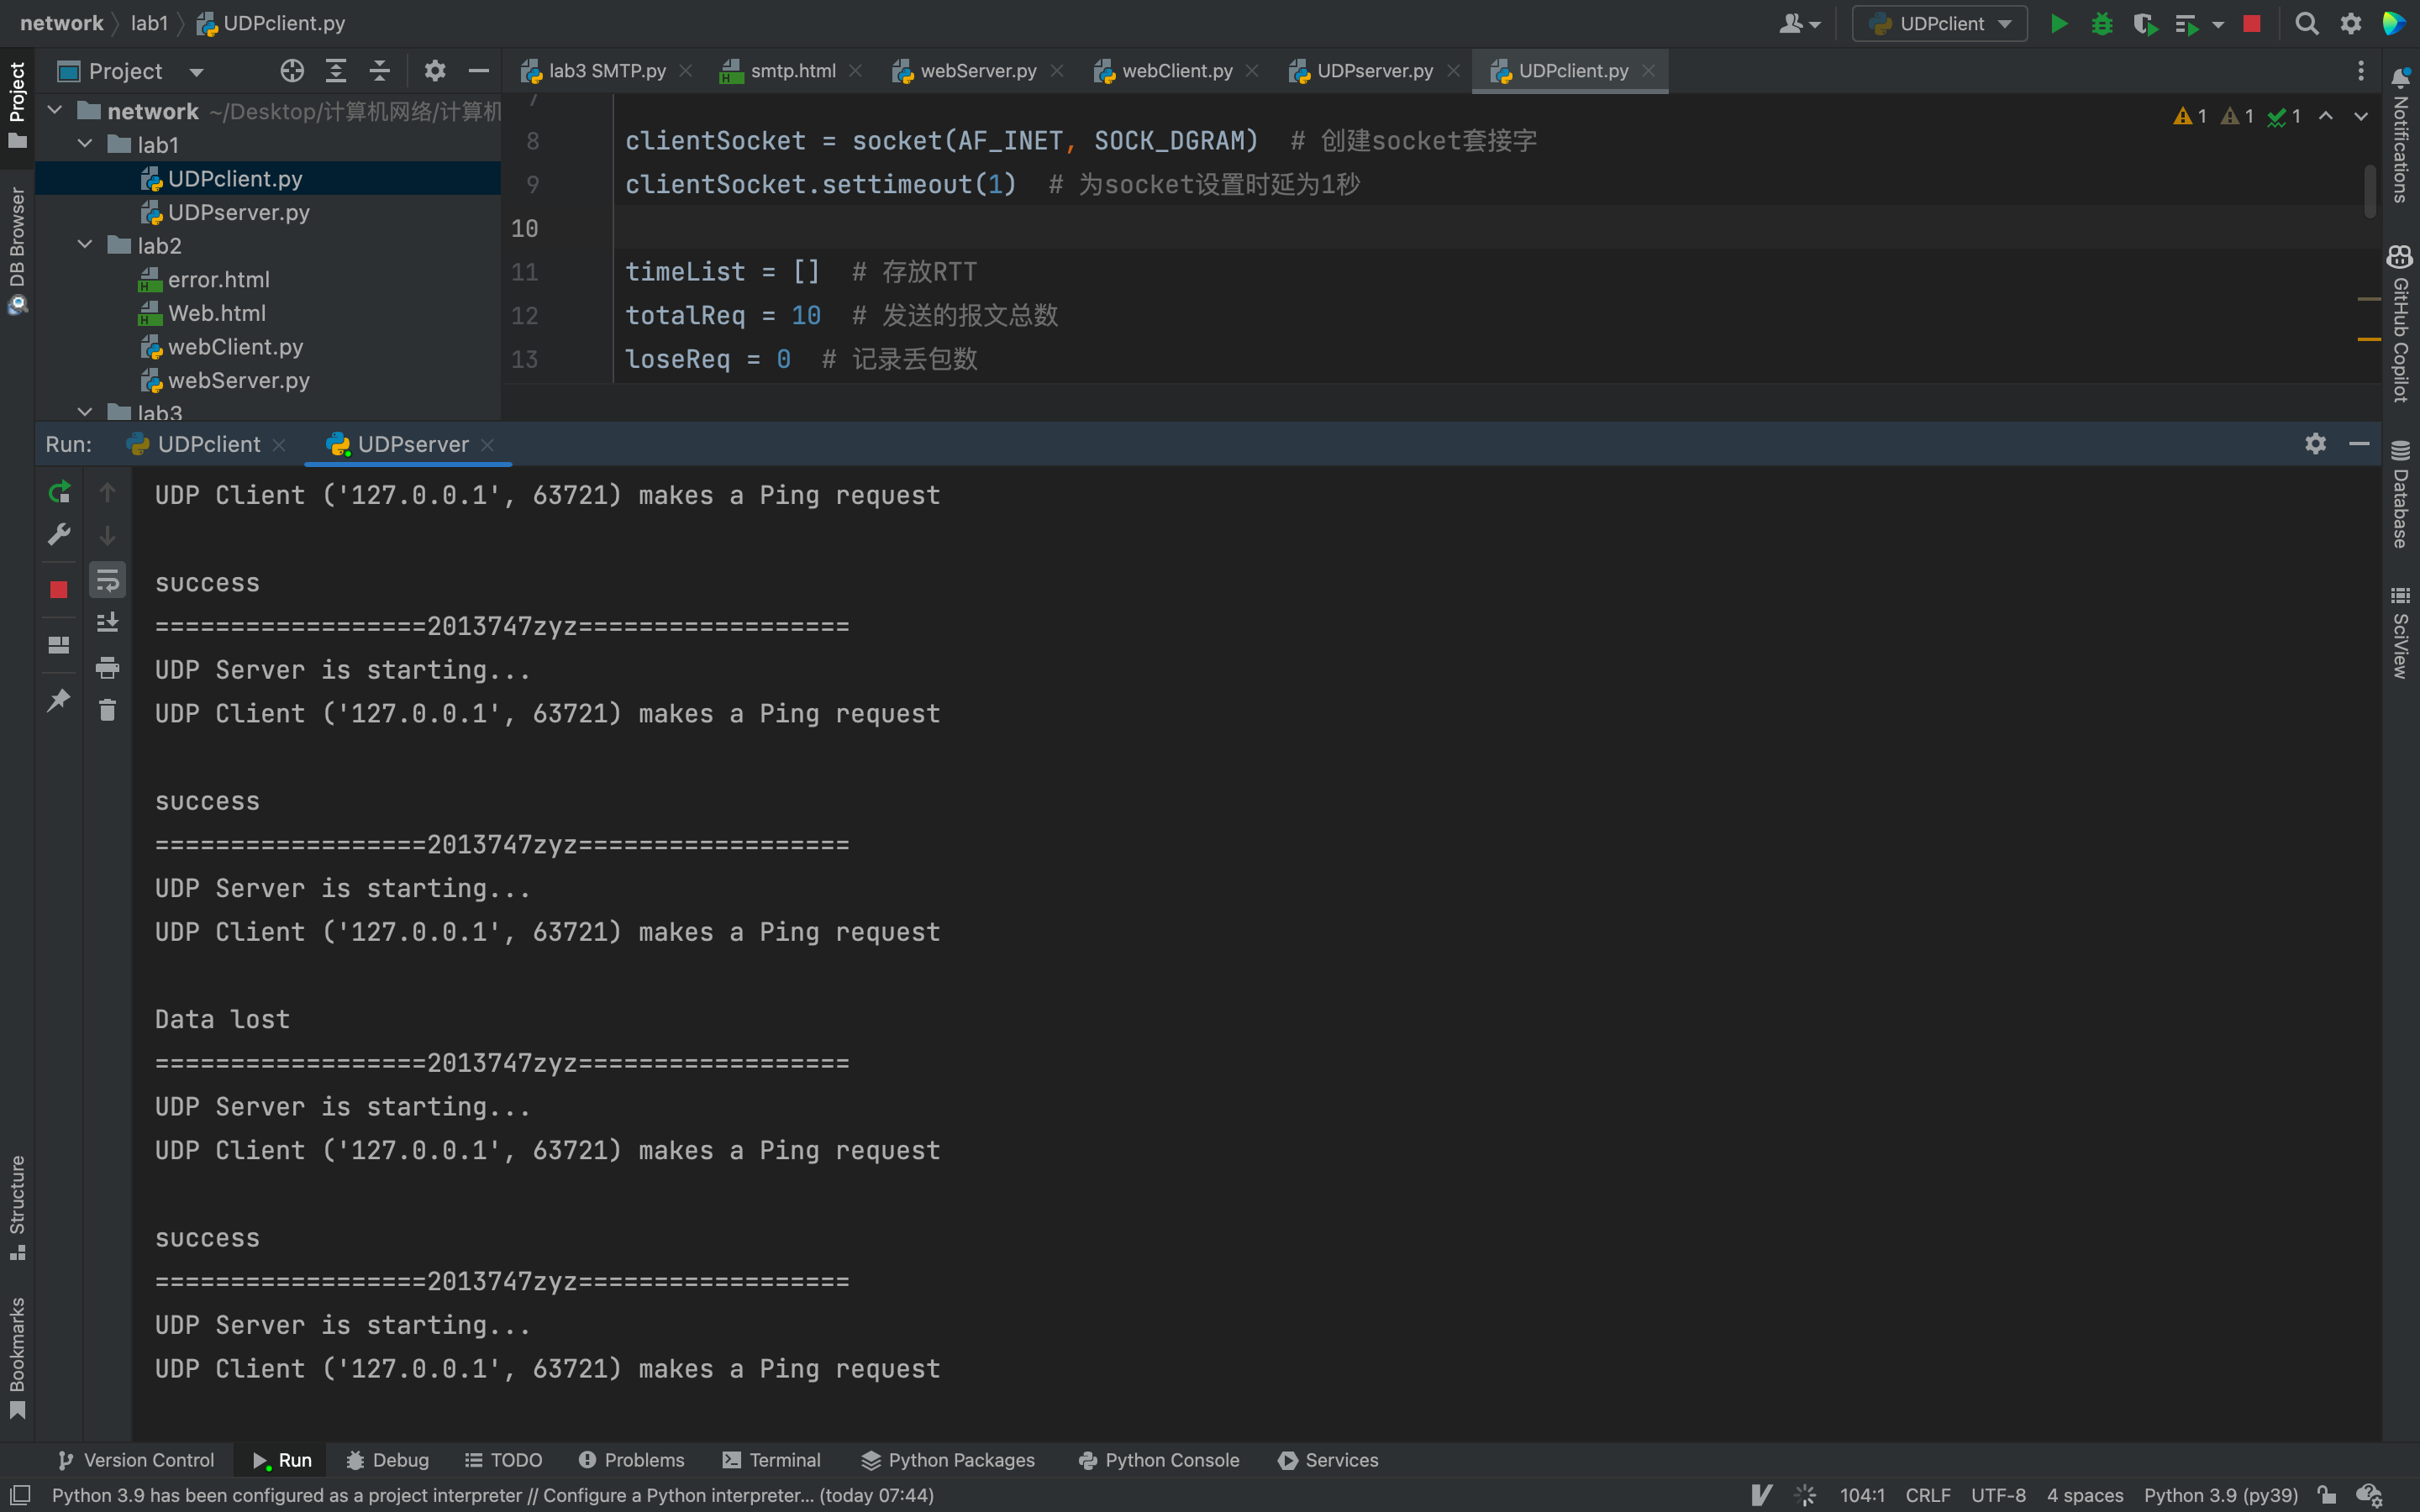
\includegraphics[width=10cm]{figure/udp_s_w.png}
\caption{UDP服务端}
\label{4}
\end{figure}

在完成代码调试后,可以尝试将客户端和服务器代码运行在不同网络环境,实现UDP Ping 的截图如图\ref{5}:
\begin{figure}[H]
  \centering
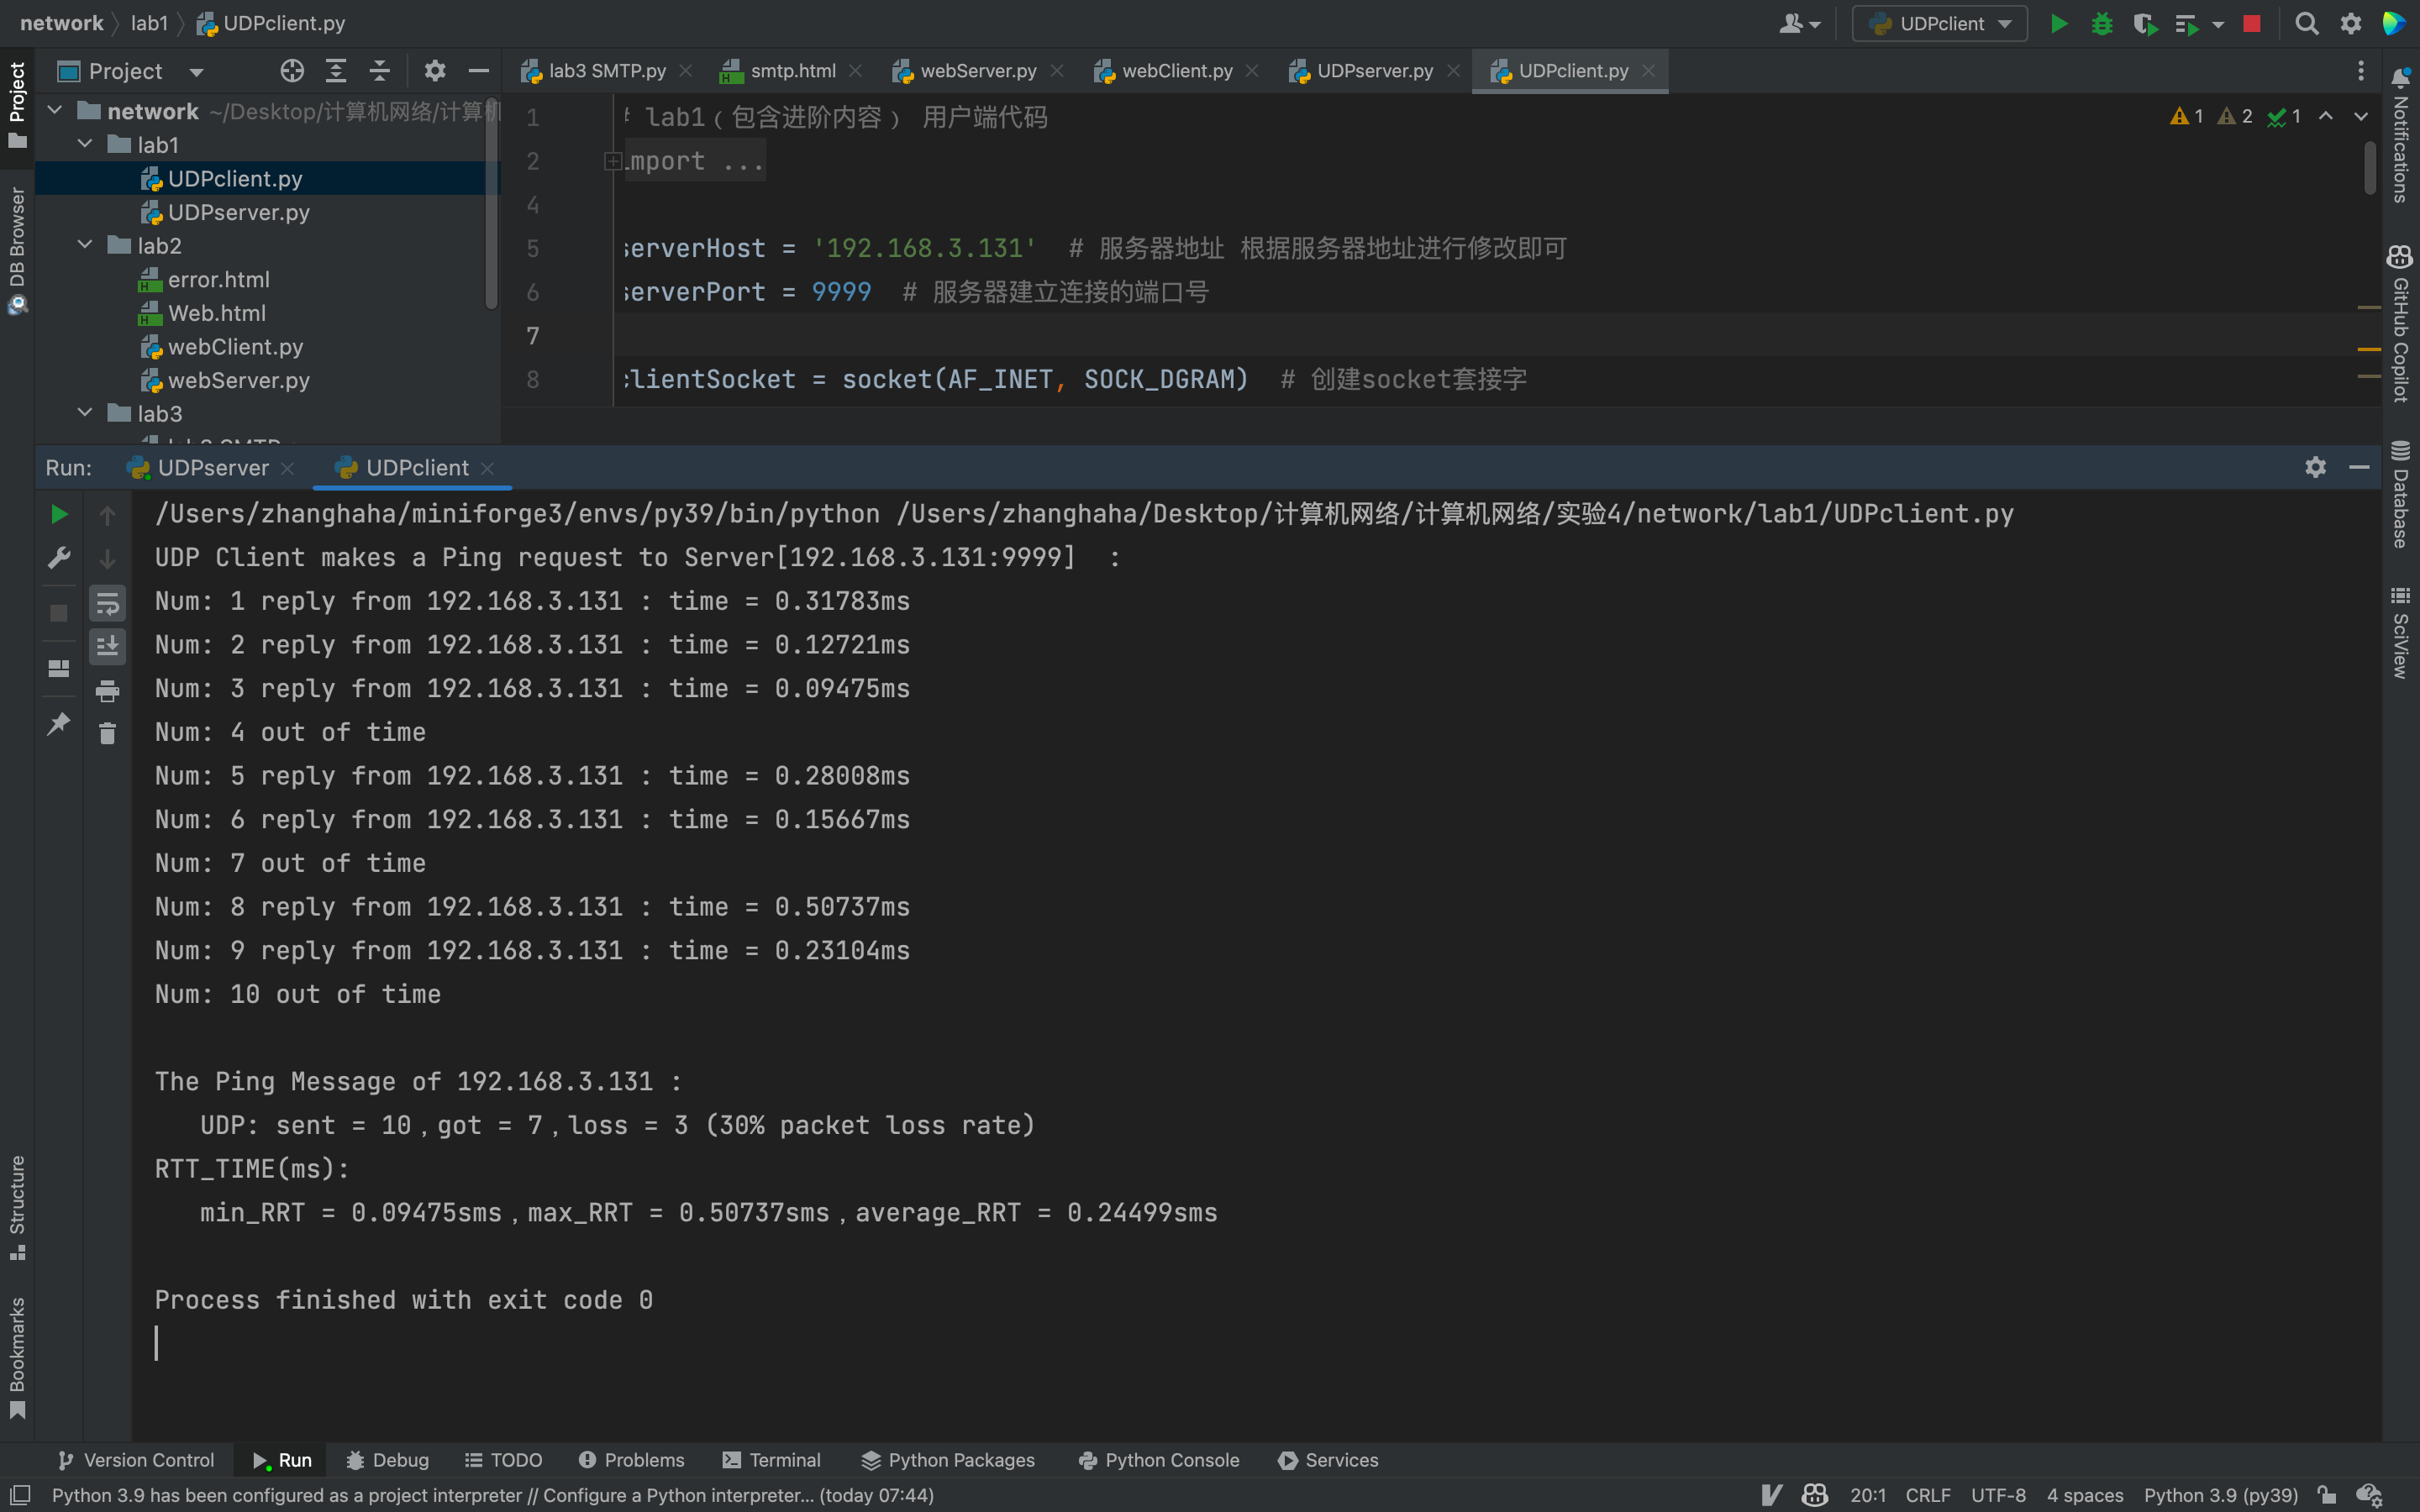
\includegraphics[width=10cm]{figure/pc_udp_c.png}
\caption{其他主机UDP客户端}
\label{5}
\end{figure}



\subsection{实验中所遇到的问题以及解决方法}
\paragraph*{RRT=0的问题} 使用time.time()得到的RRT均为0,无法达到精度要求,使用新的计时方法time.perf\_counter()得到的RRT满足精度达到要求。说明了UDP协议数据传输效率真的很高,以至于time.time()函数检测不出用时。

\subsection{实验结果分析总结}

1)UDP 是不可靠的:UDP 作为一种传输层协议,只提供了无连接通信,且不对传送的数据 包进行可靠性保证。故该程序在服务器端,模拟丢失了 30\%的客户端数据包。多次实验中, 丢包的数值不同但都存在一定的丢包率。 

2)客户端的超时机制:基于 Python 进行 UDP 消息的接收操作时,程序进入阻塞状态,未 收到数据包时,将挂起等待而不会继续执行。若运行过程中网络连接出现了问题,导致数据 包无法ࣿ时到达(本实验中在服务器端模拟丢包),这种阻塞式的工作模式将会严重的干扰程 序的执行。因此,Python 的套接字通信库提供了一种“超时”机制来防止程序卡死:提供 了一个 settimeout 方法来限制 recvfrom 的等待时间,当阻塞等待超过这个时间后仍然没有 收到数据时,程序将会抛出一个异常来说明发生了等待数据接收超时事件。 

3)UDP 数据传输速率高:从各项 RTT 中我们可以看到 UDP 的数据传输速率是相当可观的。 平常使用 windows 系统自带的 ping 命令 ping 百度时,大约需要 20ms,但在本实验中程序 不到 1ms 即可完成数据传输的一次往返过程。

4)UDP 使用场景:根据实验结果,综合得到 UDP 连接的高效但不可靠的特点,因此适用于 一次传输少量数据的应用场景。 

5)Ping 命令:在本次实验中,客户端发送 ping 消息模拟请求,服务端发送 pong 消息模拟 响应客户端的请求。使用 ping 命令,我们可以简单地判断出网络的联通状态,并大致估计 出客户端与服务端之间的 RTT,以及数据传输过程中的丢包率。
% \subsubsection{网关对pc1的arp请求}
% \begin{figure}[h!]
%   \centering
%   \begin{subfigure}[b]{0.3\linewidth}
%     
\includegraphics[width=\linewidth]{figure/nankai.jpg}
%     \caption{观察PC1与Sw3之间.}
%   \end{subfigure}
%   \begin{subfigure}[b]{0.6\linewidth}
%     
\includegraphics[width=\linewidth]{figure/nankai.jpg}
%     \caption{使用WireShark抓取数据包.}
%   \end{subfigure}
%   \caption{使用WireShark抓取PC1与Sw3之间的数据包.}
%   \label{fig:128}
% \end{figure}


\section{TCP 通信与 Web 服务器}

\subsection{实验目的}
熟悉基于 Python 进行 TCP 套接字编程的基础知识,理解 HTTP 报文格式,能基于 Python 编写 一个可以一次响应一个 HTTP 请求,并返回静态文件的简单 Web 服务器。

\subsection{实验内容}
利用 Python 开发一个可以一次处理一个 HTTP 请求的 Web 服务器,该服务器可以接受并解析 HTTP 请求,然后从服务器的文件系统中读取被 HTTP 请求的文件,并根据该文件是否存在而向客 户端发送正确的响应消息。

\paragraph*{进阶内容}
实现了一个能同时处理多个请求的多线程服务器。


\subsection{实验原理}
基于 TCP 的面向客户端/服务器在 Python 实现中的的工作流程是:

1. 首先在服务器端通过调用socket()创建套接字来启动一个服务器;

2. 服务器调用bind()绑定指定服务器的套接字地址(IP 地址 + 端口号);

3. 服务器调用listen()做好侦听准备,同时规定好请求队列的长度;

4. 服务器进入阻塞状态,等待客户的连接请求;

5. 服务器通过accept()来接收连接请求,并获得客户的 socket() 地址。

6. 在客户端通过调用socket()创建套接字;

7. 客户端调用connect()和服务器建立连接。

8. 连接建立成功后,客户端和服务器之间通过调用read()和write()来接收和发送数据。

9. 数据传输结束后,服务器和客户各自通过调用close()关闭套接字。

在不同的计算机语言实现中,上述调用的名字和具体工作流程可能略有不同。
基于 Python 的 TCP 客户端/服务器具体工作流程如图所示。

\begin{figure}[H]
  \centering
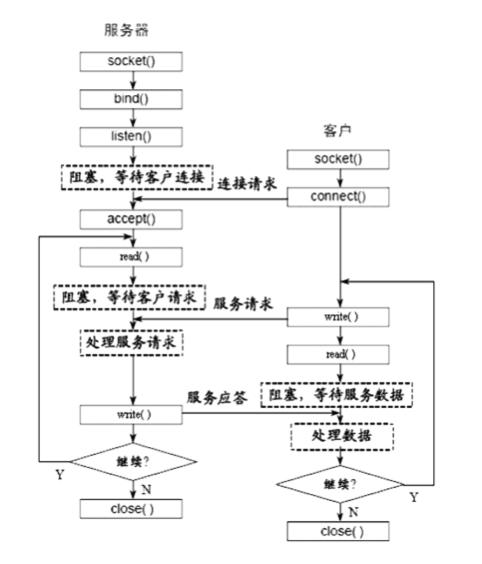
\includegraphics[width=10cm]{figure/2.png}
\caption{面向连接客户/服务器流程图}
\label{2}
\end{figure}

\subsection{实验过程与截图(含进阶任务)}
完成一个具有以下功能的简单 Web 服务器:

1. 服务器收到请求时能创建一个 TCP 套接字;

2. 可以通过这个 TCP 套接字接收 HTTP 请求;

3. 解析 HTTP 请求并在操作系统中确定客户端所请求的特定文件;

4. 从服务器的文件系统读取客户端请求的文件;

5. 当被请求文件存在时,创建一个由被请求的文件组成的“请求成功”HTTP 响应报文;

6. 当被请求文件不存在时,创建“请求目标不存在”HTTP 响应报文;

7. 通过 TCP 连接将响应报文发回客户端;

8. 实现一个能够同时处理多个请求的多线程服务器。

\paragraph*{TCP Server}
TCP Server可以同时处理多个请求:
为使得服务器能够同时处理多个请求,需要在服务器端创建多个线程和套接字来处理请求。
首先创建一个 serverSocket 的套接字,用于监听连接。
每当 serverSocket 接收到 一个客户端请求时,就建立一个 connectionSocket 连接,
同时使用 threading.Thread 和 start 方法创建并启动一个线程,
该线程使用 connectionSocket 完成向客户端传输数据的任务,
而 serverSocket 继续等待其他新客户端的连接。

代码如下:
\begin{spacing}{1}  
	\begin{lstlisting}[language={Python}]
    # lab2 服务端代码
    import threading
    import time
    from socket import *
    
    # 本机
    HOST = '10.10.1.203'  # 服务器地址 根据实际情况进行修改即可
    # 开放的端口
    PORT = 9999
    # 成功请求的HTTP头部
    head = 'HTTP/1.x 200 OK\r\nContent-Type: text/html\r\n'+'Server:'+HOST+'-'+str(PORT)+'\r\n\r\n'
    lock = threading.Lock()
    
    def handle_client(connectionSocket, address):
        # 获取client请求的文件名及在本机sever上的路径
        lock.acquire()
        print("=================2013747zyz=======================")
        message = connectionSocket.recv(1024).decode()
        print("receive message time:", time.strftime("%Y-%m-%d %H:%M", time.localtime(time.perf_counter())), sep="")
        filename = message.split()[1]
        filepath = filename[1:]
        print('TCP Client', address, 'Request File: ', filepath)
        try:
            f = open(filepath)
            outputdata = head + f.read()
            f.close()
            connectionSocket.sendall(outputdata.encode())
            connectionSocket.close()
            print("Success!")
        except:
            print("[ERROR]The file being fetched is not existed.")
            with open("error.html", "r") as f:  # 异常则打开异常响应文件(404)
                outputdata = head + f.read()
            f.close()
            connectionSocket.sendall(outputdata.encode())
            connectionSocket.close()
            print("Wrong!")
        lock.release()
    
    def server():
        # 准备服务器端socket
        serverSocket = socket(AF_INET, SOCK_STREAM)
        # 连接
        serverSocket.bind((HOST, PORT))
        # 监听
        serverSocket.listen(10)
        print("TCP Server is listening...\n")
        while True:
            # 建立连接
            # 如果有新的客户端来链接服务端,那么就产生一个新的套接字专门为这个客户端服务
            # connectionSocket用来为这个客户端服务
            # serverSocket专门等待其他新的客户端连接
            connectionSocket, address = serverSocket.accept()
            # 设置线程,调用handle_client处理获取到的每一个用户端请求
            new_thread = threading.Thread(target=handle_client, args=(connectionSocket, address))
            # 启动线程
            new_thread.start()
        serverSocket.close()
    
    
    if __name__ == '__main__':
        server()
    
		\end{lstlisting}
\end{spacing}

\paragraph*{TCP Client}
TCP Client可以实现多线程的TCP客户端,可以同时发出多个请求:
测试多线程 Web 服务器时,编写了一个模拟并发请求的客户端程序,该客户端程序创建 了 threadNum 个线程,每个线程均向服务器请求 HelloWorld.html 文件。

代码如下:
\begin{spacing}{1}  
	\begin{lstlisting}[language={Python}]
    # lab2 用户端代码
    import threading
    from socket import *
    
    # 需要访问的服务器地址
    serverHOST = '127.0.0.1'  # 服务器地址 根据实际情况修改即可
    # 服务器开放的端口
    serverPORT = 9999
    # 总共有多少个客户端线程发出请求
    threadNum = 5
    CODE = 'utf-8'
    url = '/Web.html'
    
    def send_data(rank):
        socketClient = socket(AF_INET, SOCK_STREAM)
        socketClient.connect((serverHOST, serverPORT))
        request_url = 'GET {} / HTTP/1.1\r\n' \
                      'Accept: text/html' \
                      'Host: {}\r\n ' \
                      'Connection: Close\r\n\r\n'.format(url, serverHOST + ':' + str(serverPORT))
        socketClient.send(request_url.encode(CODE))
        response = socketClient.recv(1024).decode()
        print('Client Number:', rank, '\nTCP Server reply:\n', response)
        print('=======================================================')
        socketClient.close()
    
    
    def client():
        for rank in range(0, threadNum):
            p = threading.Thread(target=send_data, args=(rank,))
            p.start()
        pass
    
    
    if __name__ == '__main__':
        client()
    
		\end{lstlisting}
\end{spacing}

当被请求文件存在时,创建一个由被请求的文件组成的“请求成功”HTTP 响应报文,如图\ref{7},\ref{8}:
\begin{figure}[H]
  \centering
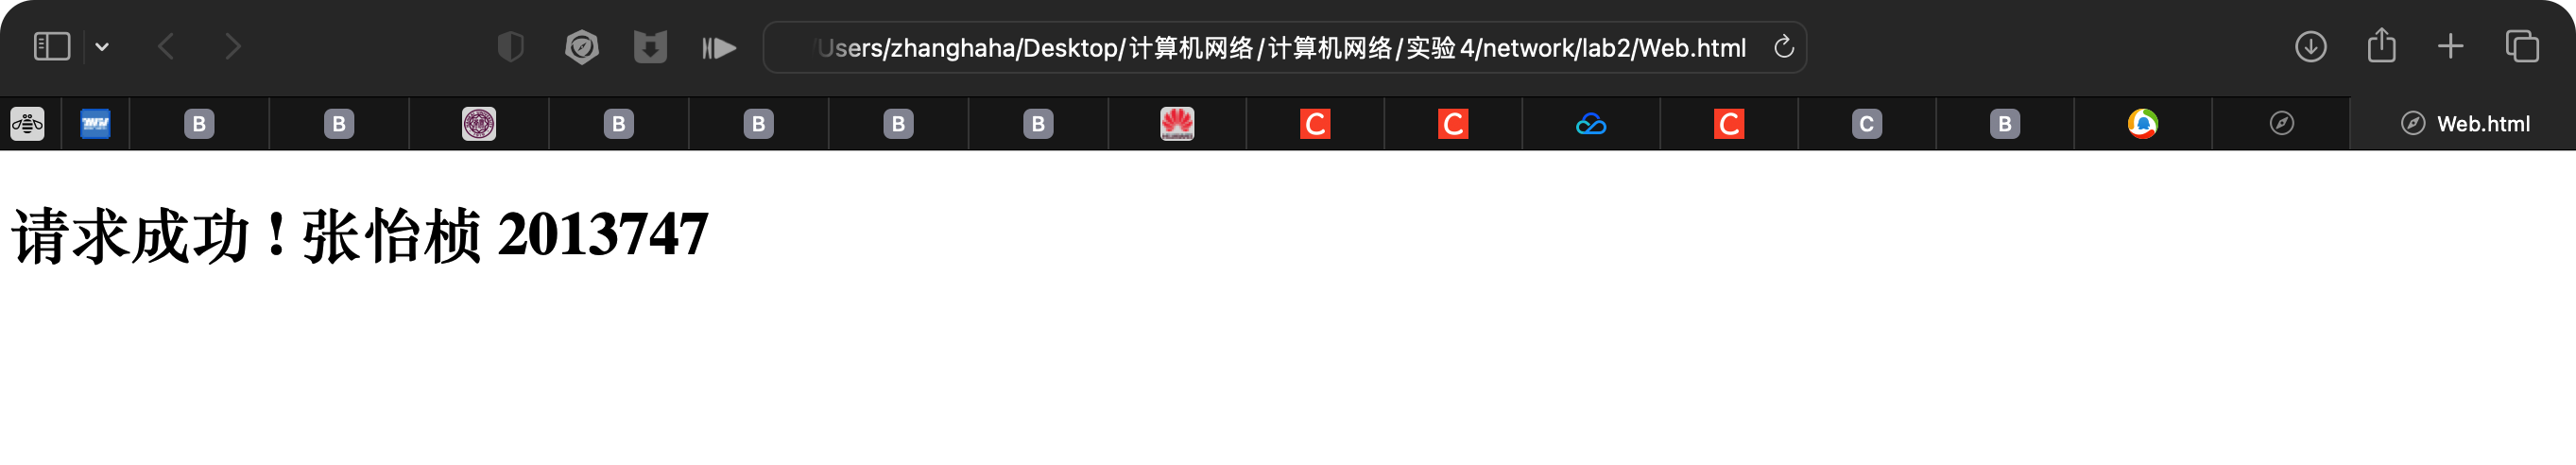
\includegraphics[width=12cm]{figure/web.png}
\caption{请求成功获得的信息}
\label{web}
\end{figure}

\begin{figure}[H]
  \centering
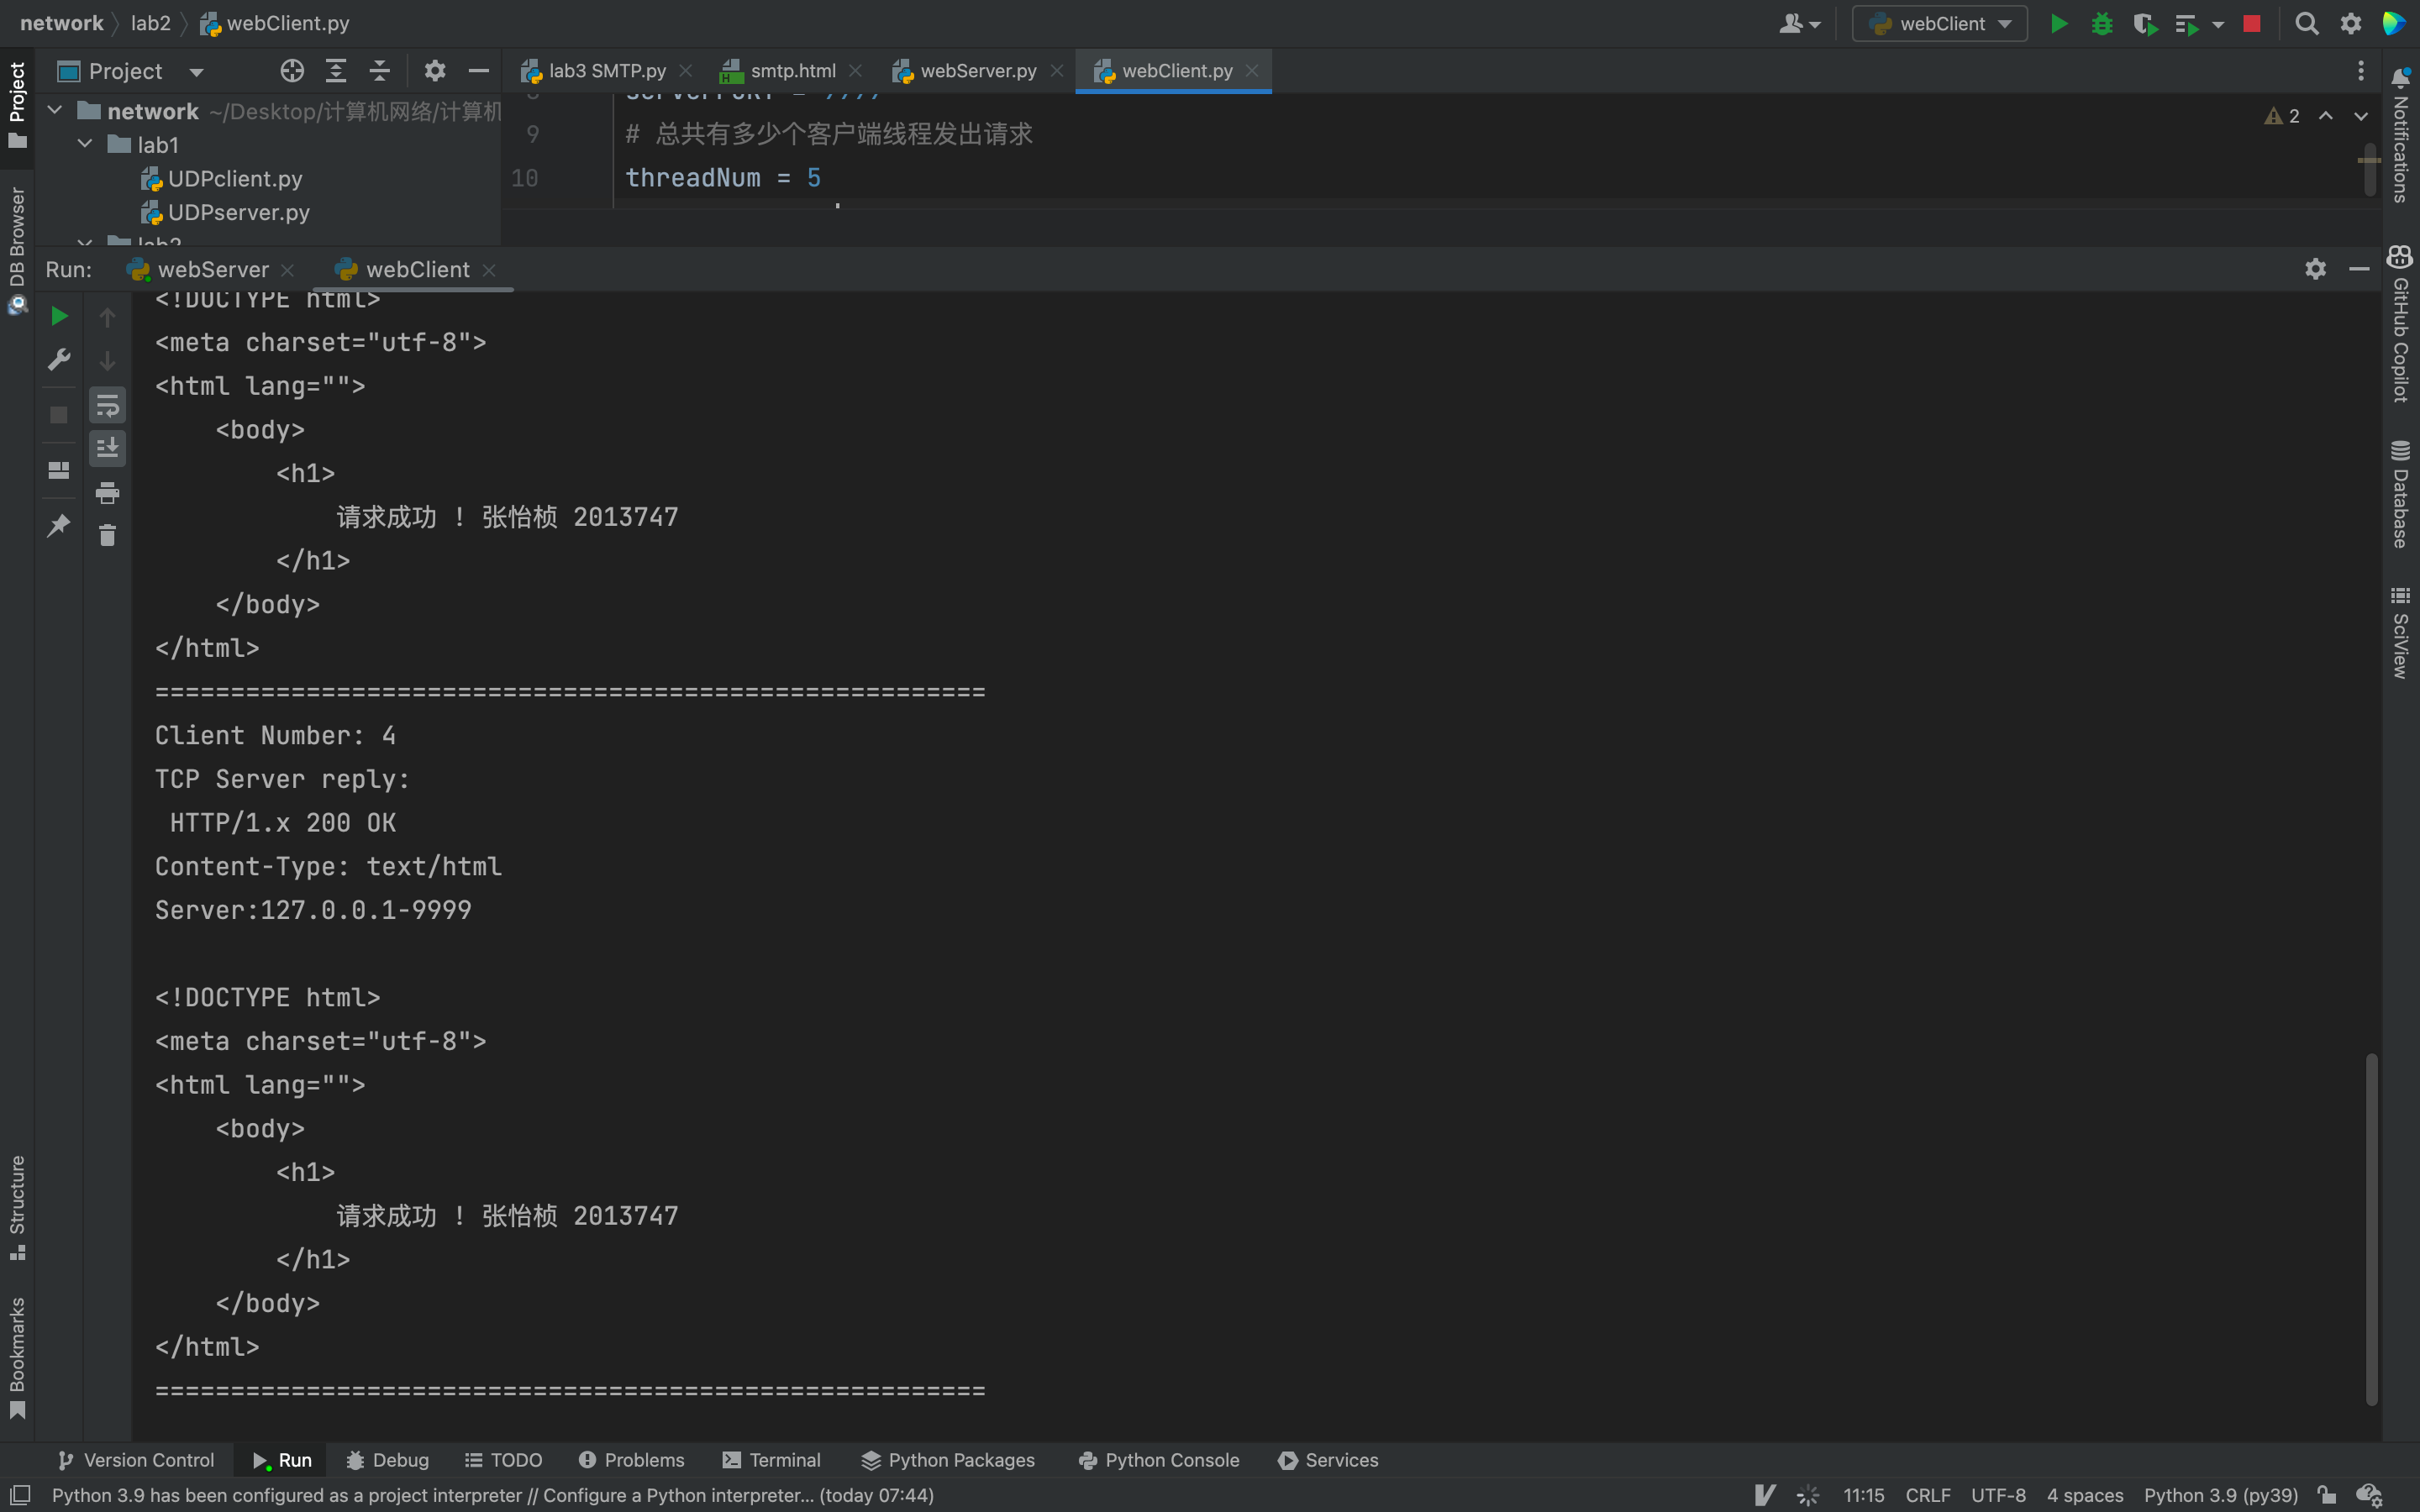
\includegraphics[width=10cm]{figure/tcp_c_s.png}
\caption{TCP Server 请求成功}
\label{7}
\end{figure}

\begin{figure}[H]
  \centering
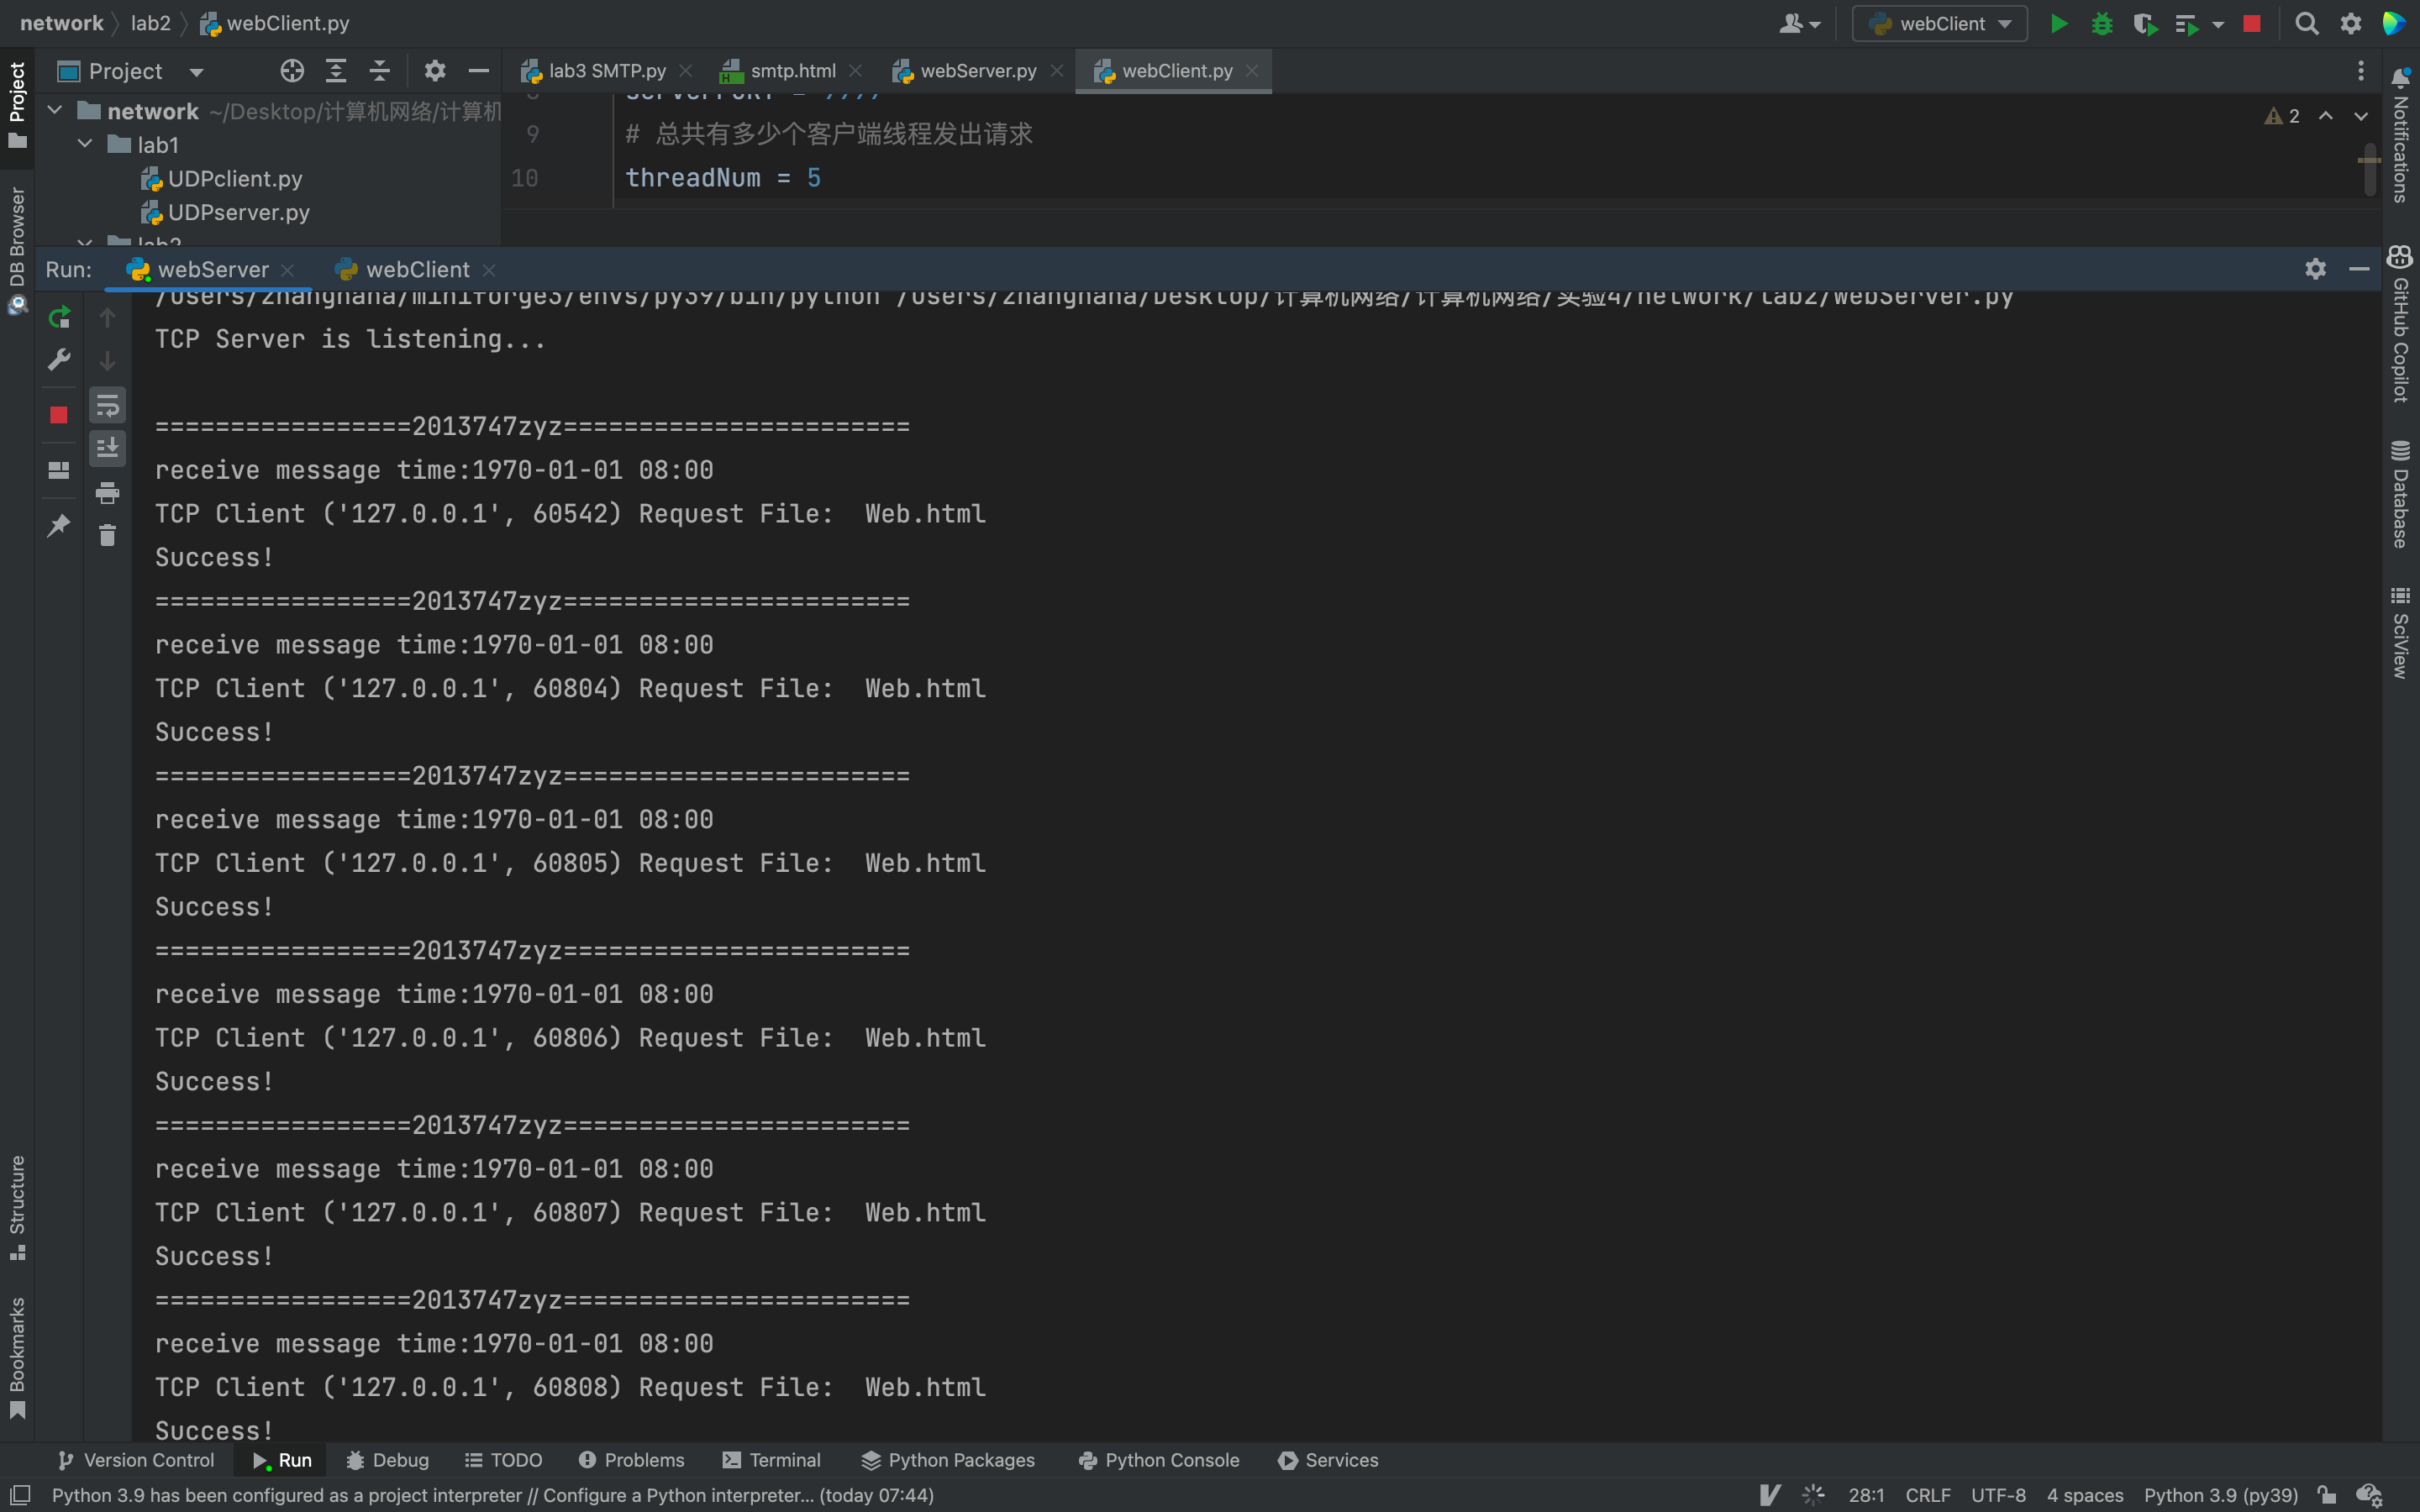
\includegraphics[width=10cm]{figure/tcp_s_s.png}
\caption{TCP Client 请求成功}
\label{8}
\end{figure}

当被请求文件不存在时,创建“请求目标不存在”HTTP 响应报文,如图\ref{9},\ref{10}:
\begin{figure}[H]
  \centering
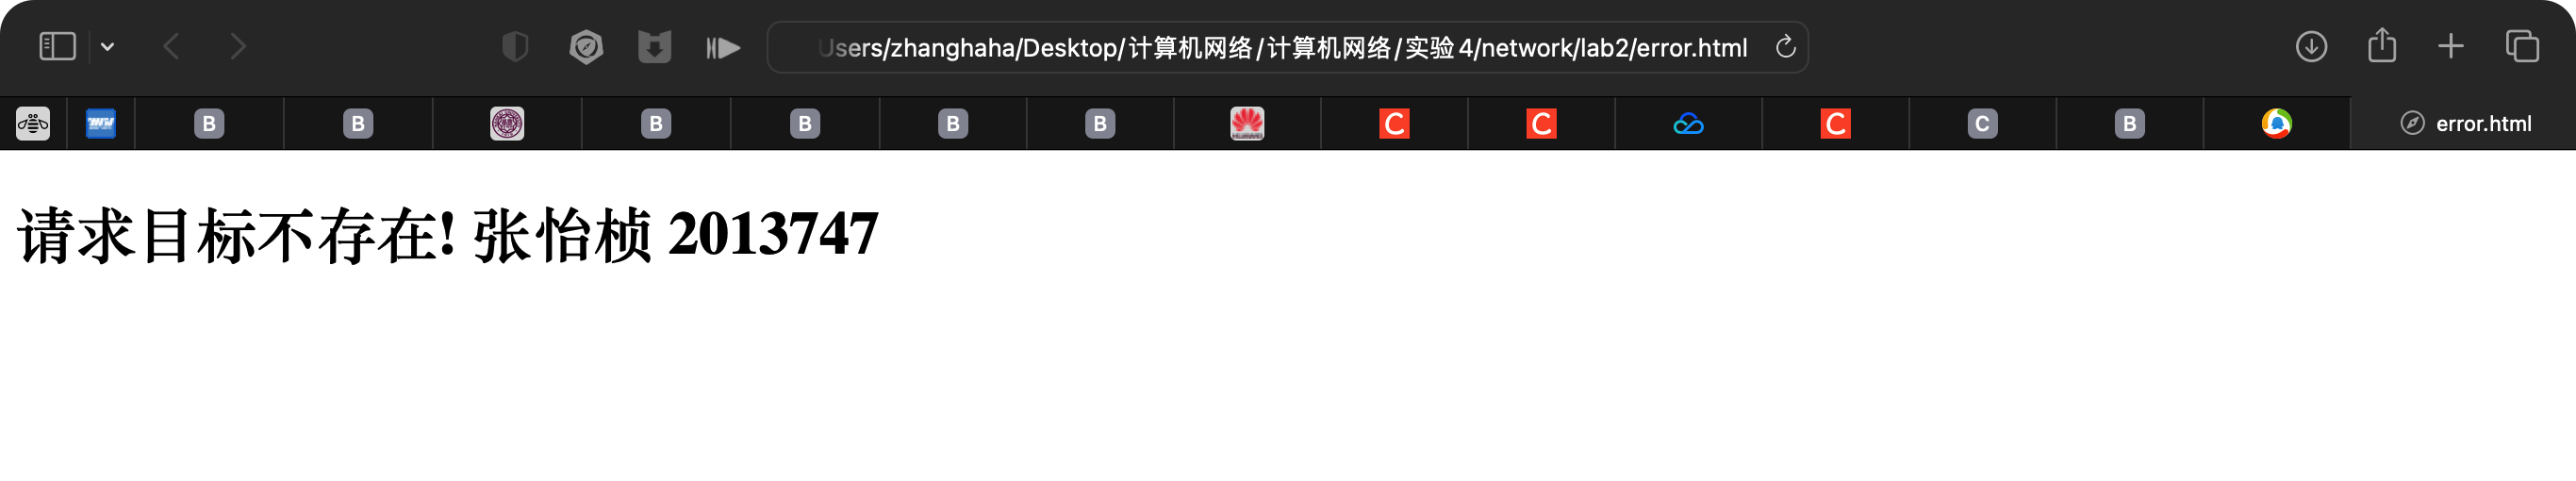
\includegraphics[width=12cm]{figure/error.png}
\caption{请求失败获得的信息}
\label{error}
\end{figure}

\begin{figure}[H]
  \centering
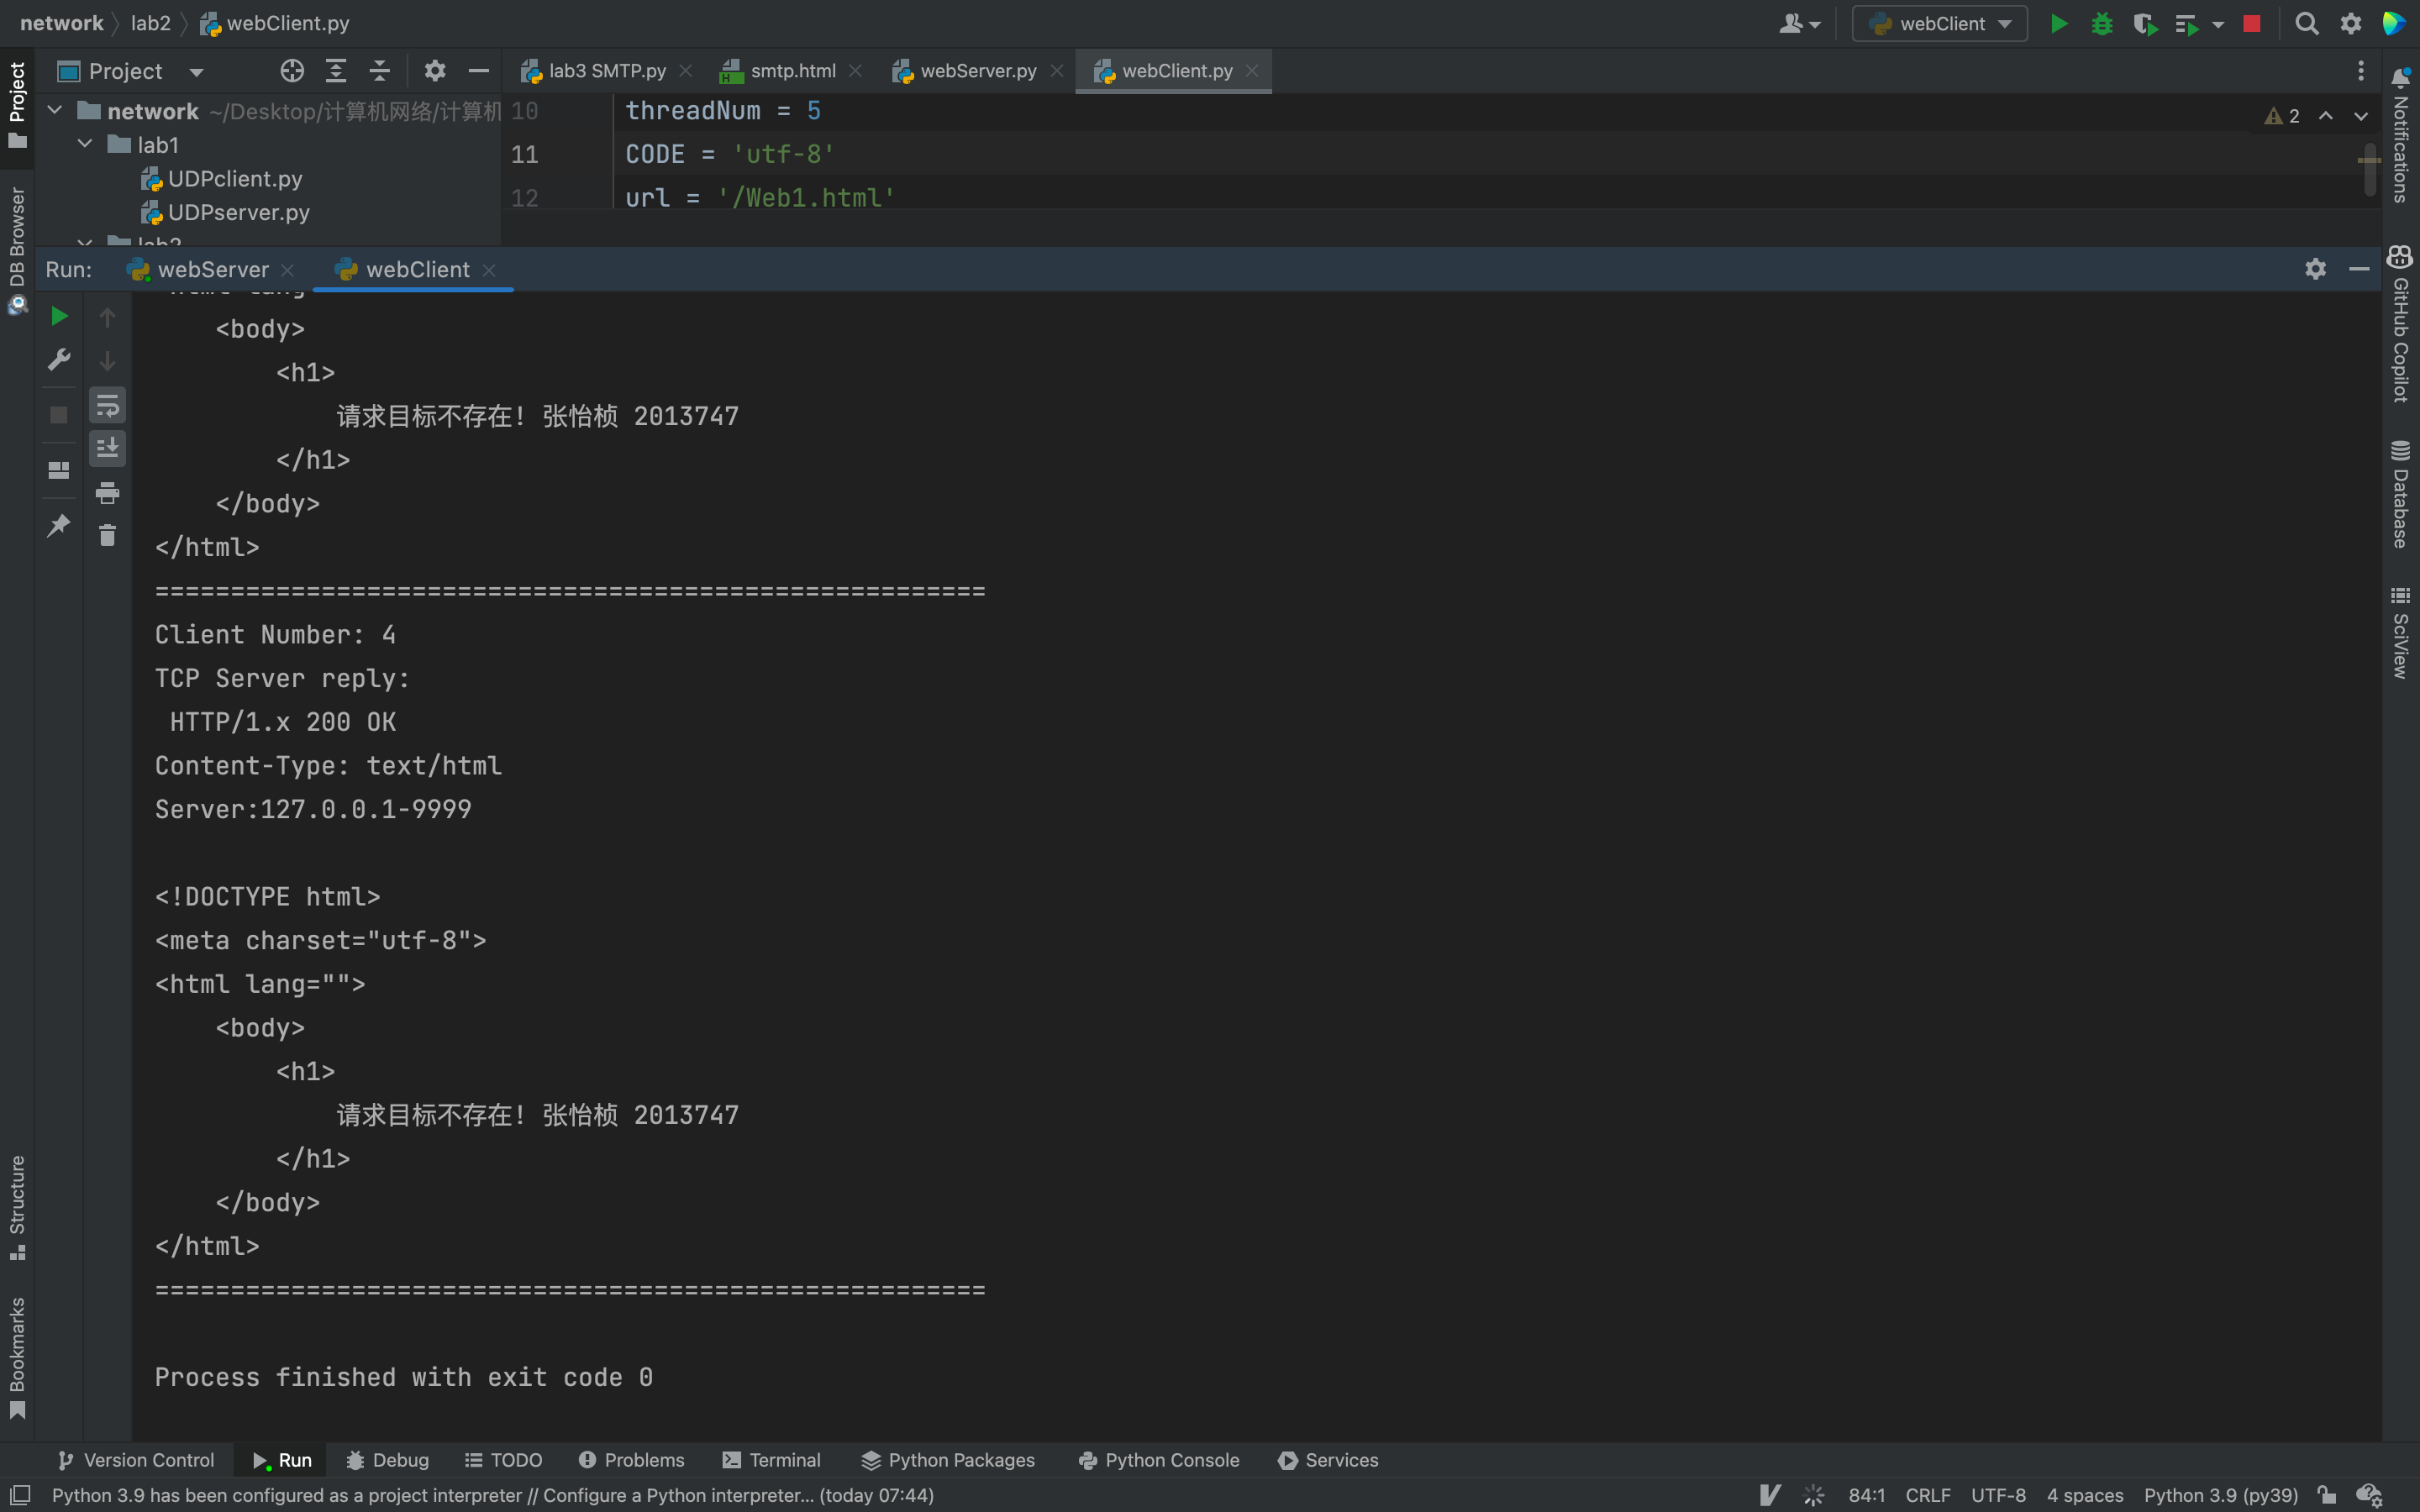
\includegraphics[width=10cm]{figure/tcp_c_w.png}
\caption{TCP Server 请求失败}
\label{9}
\end{figure}

\begin{figure}[H]
  \centering
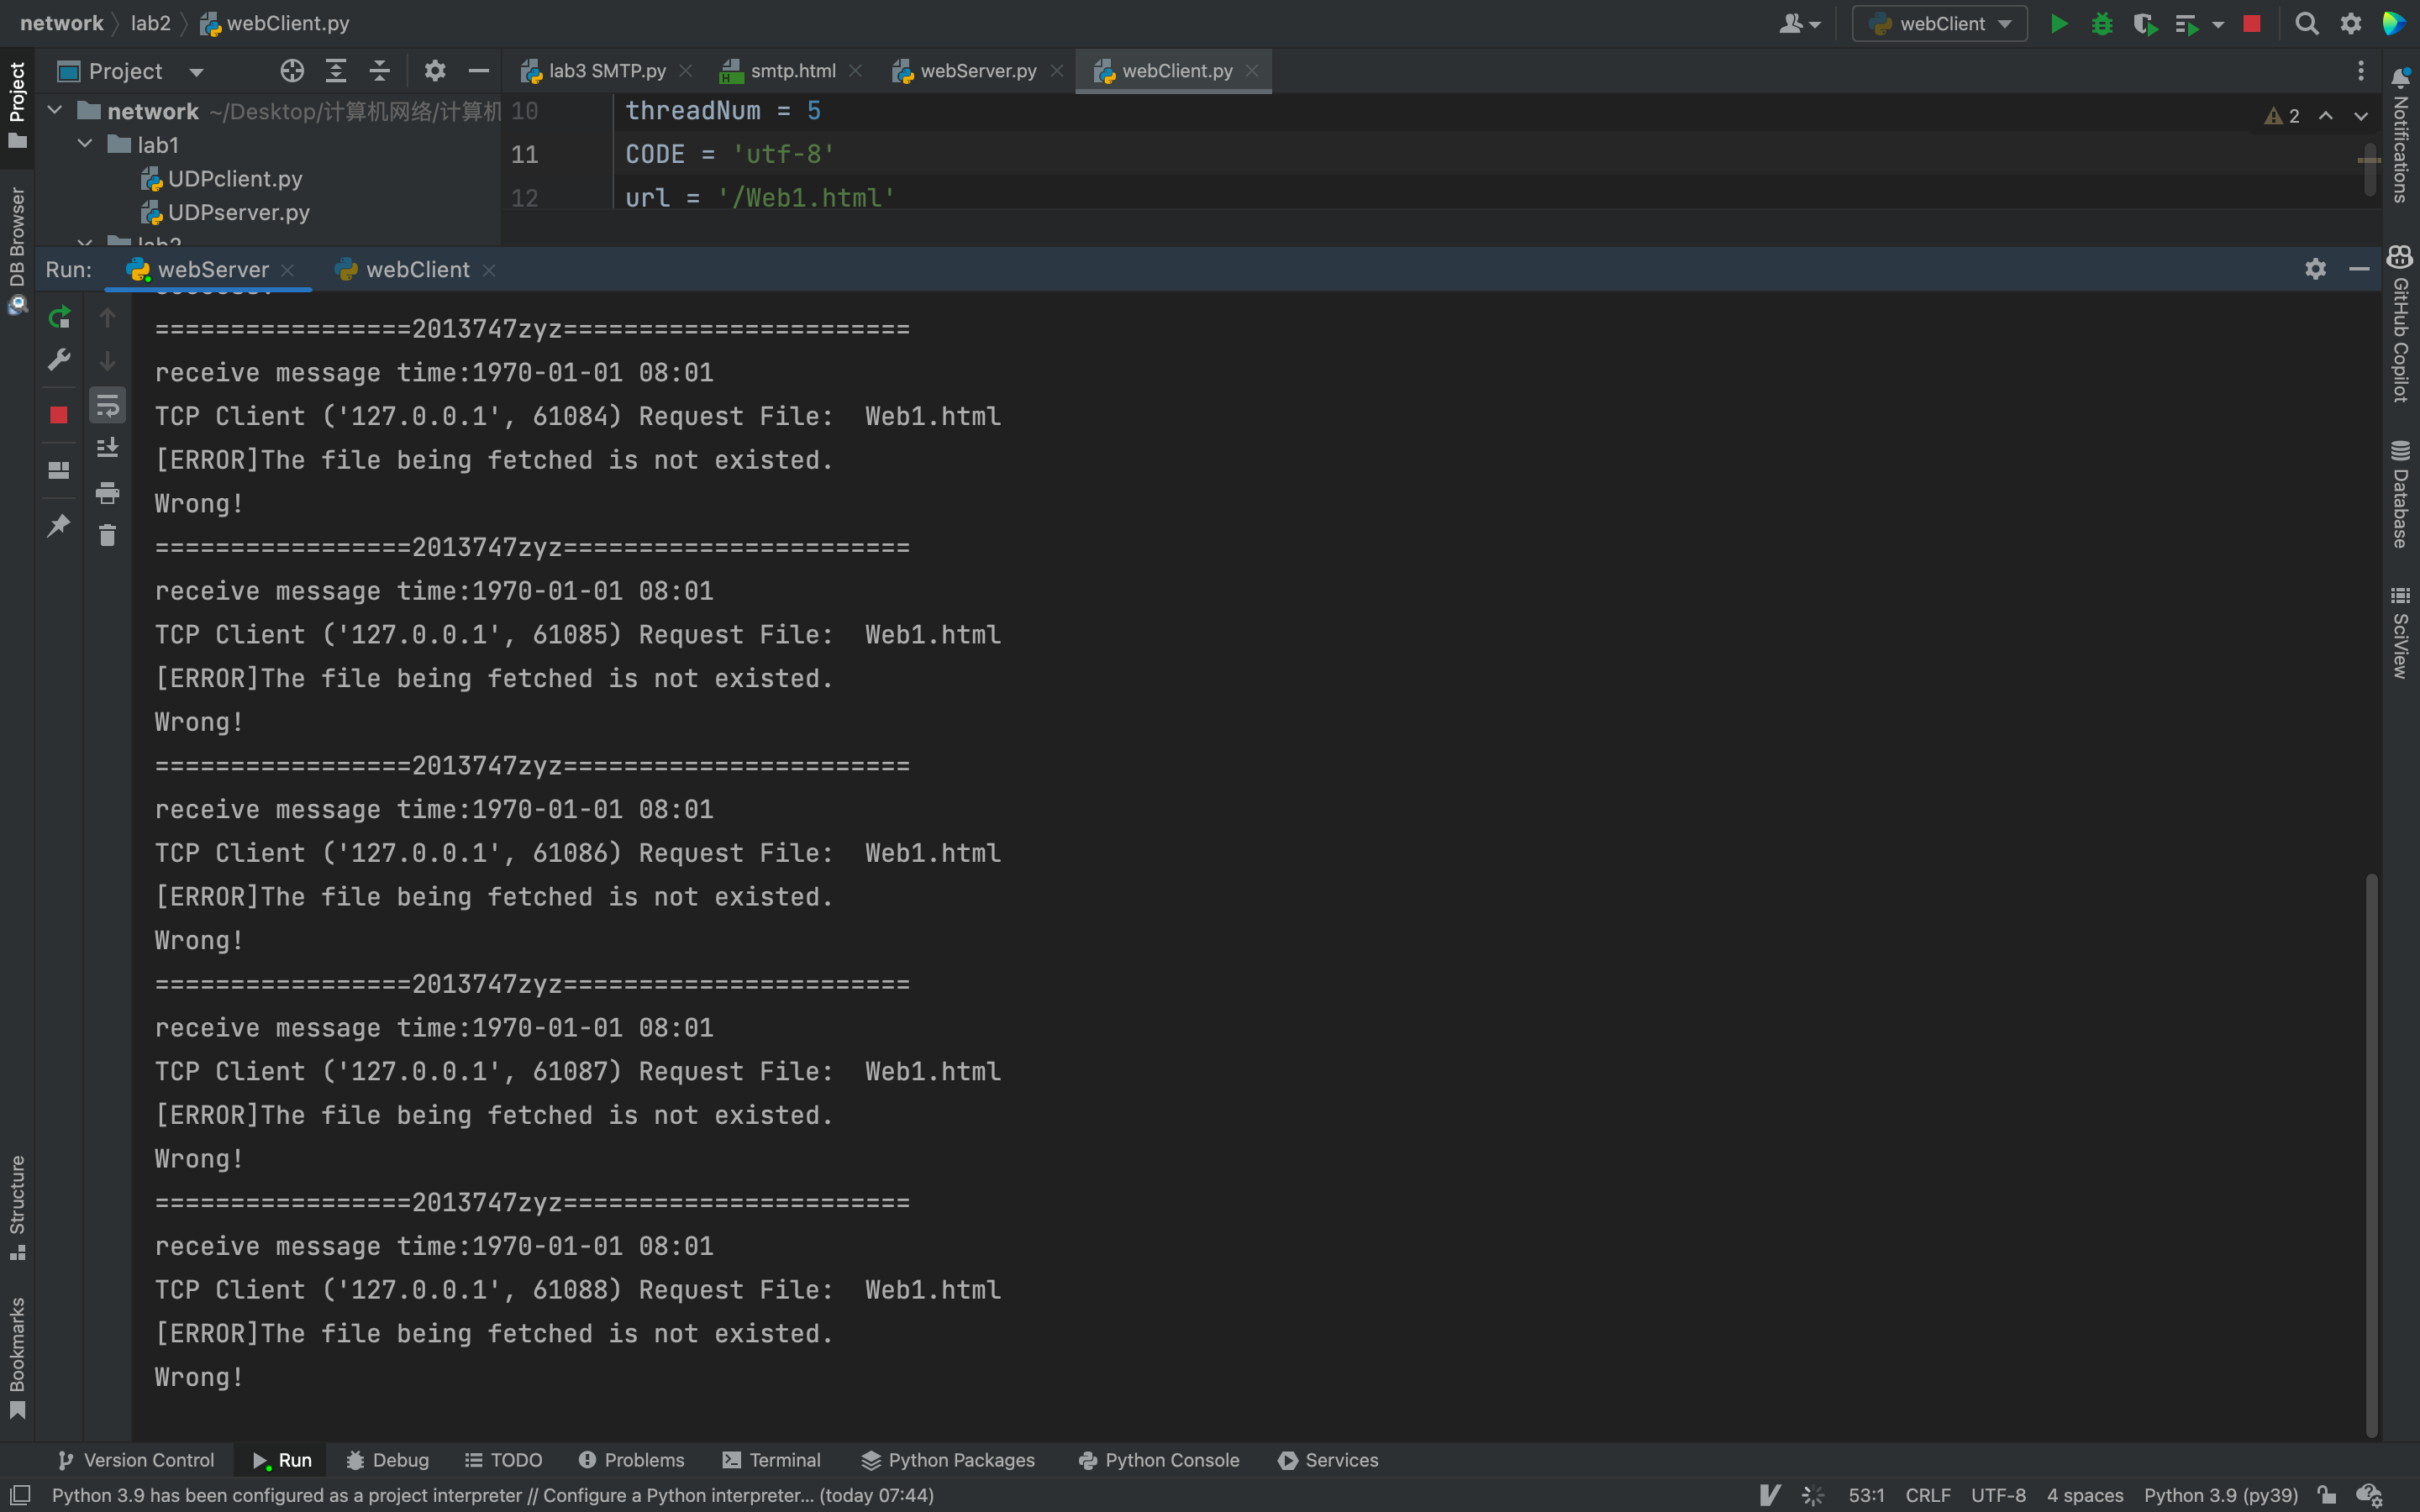
\includegraphics[width=10cm]{figure/tcp_s_w.png}
\caption{TCP Client 请求失败}
\label{10}
\end{figure}

在本机上先运行多线程 Web 服务器程序,再运行上述模拟客户端发送并发请求的测试程序, 服务器端和模拟客户端的运行结果如图\ref{11},\ref{12}:
\begin{figure}[H]
  \centering
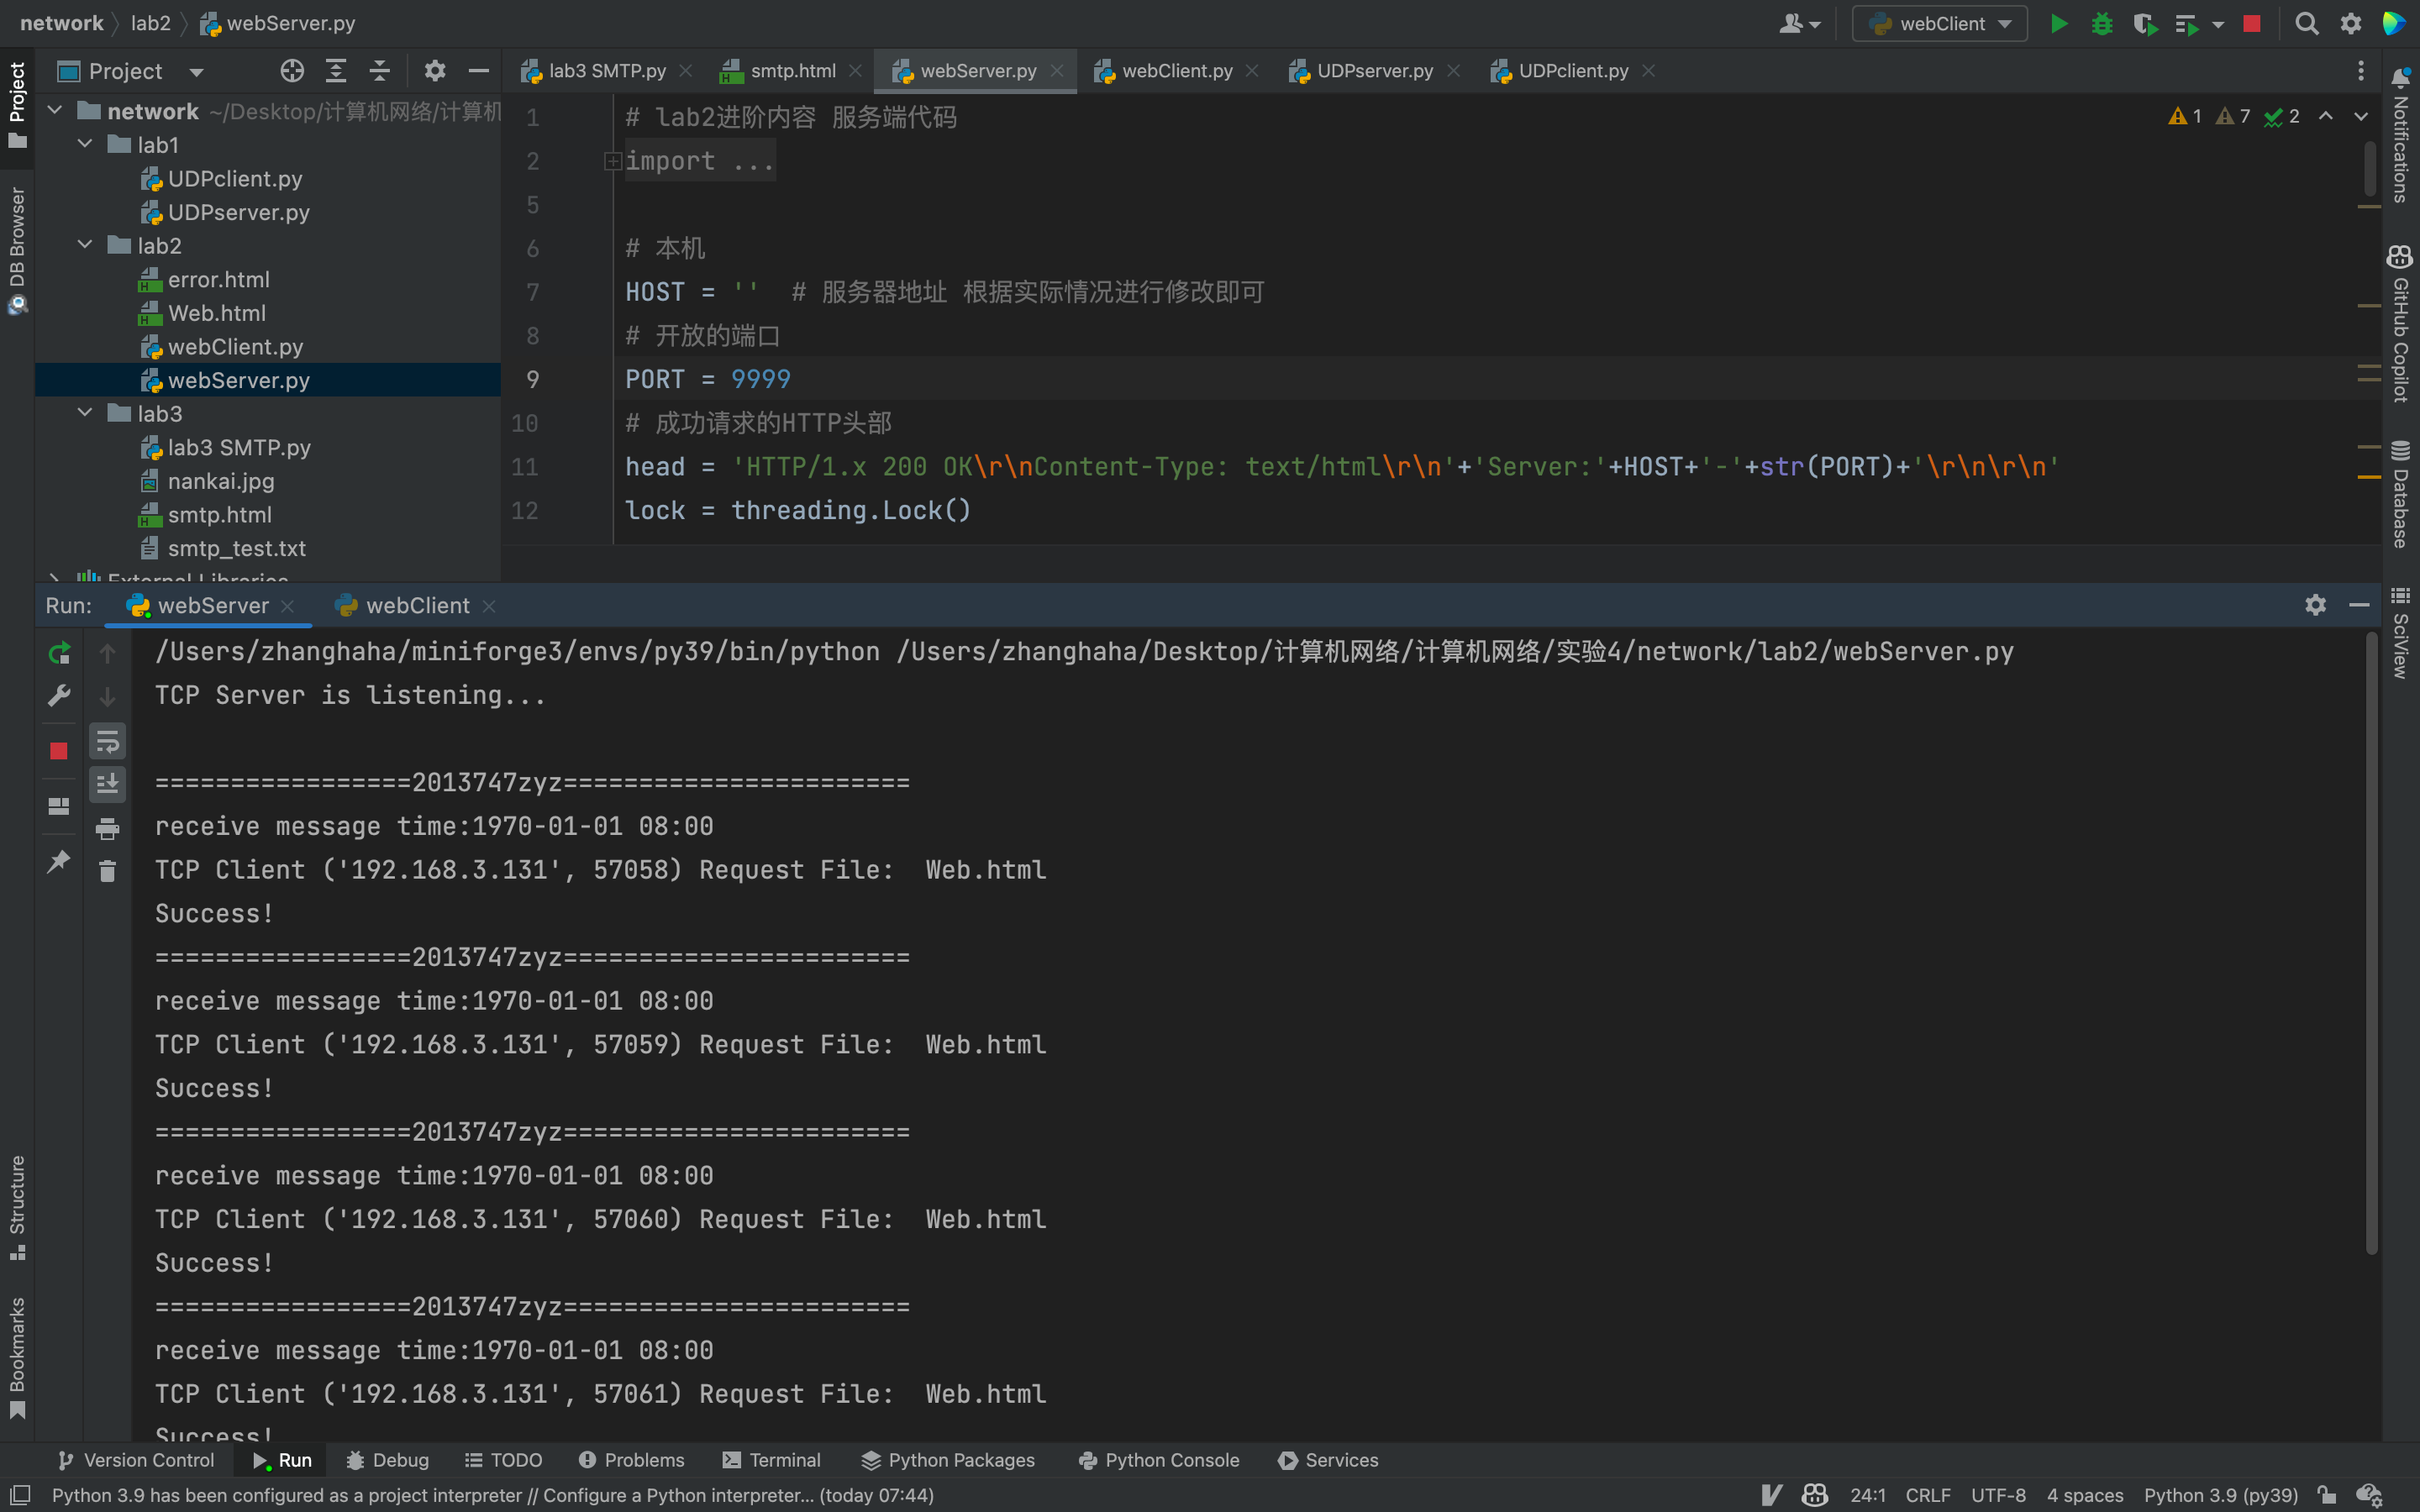
\includegraphics[width=10cm]{figure/22.png}
\caption{其他主机TCP Server}
\label{11}
\end{figure}

\begin{figure}[H]
  \centering
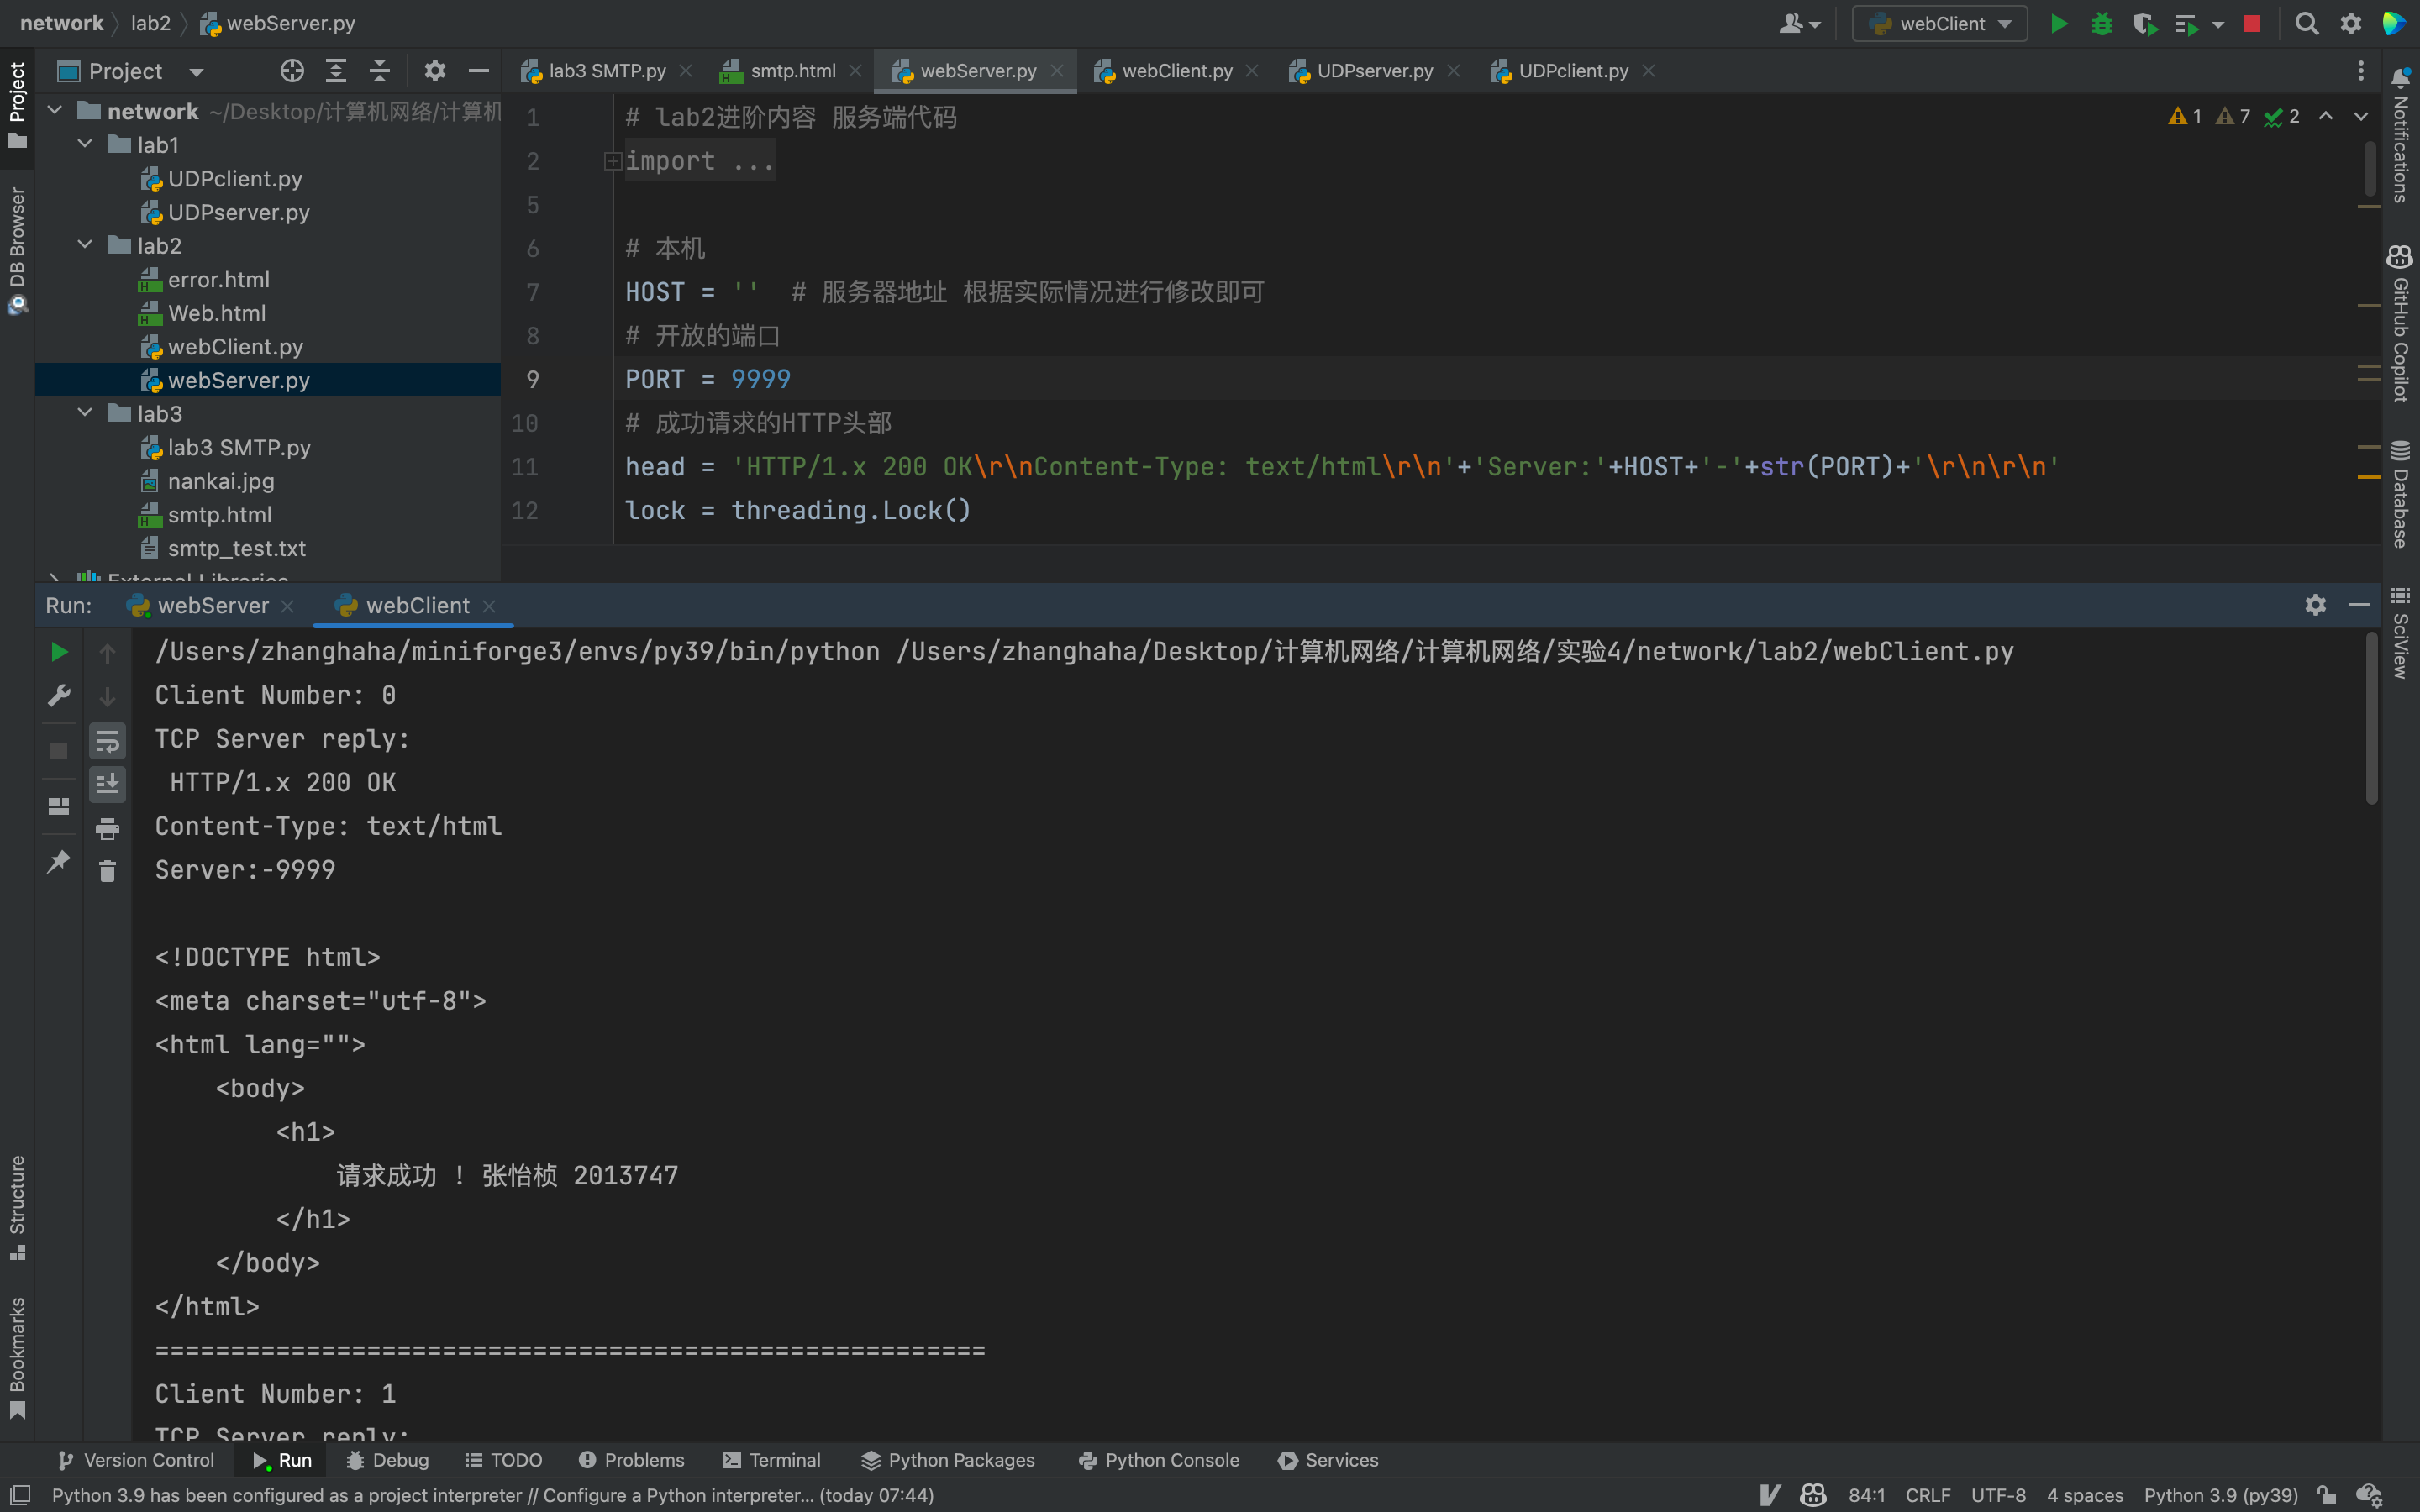
\includegraphics[width=10cm]{figure/11.png}
\caption{其他主机TCP Client}
\label{12}
\end{figure}

\subsection{实验中所遇到的问题以及解决方法}
在实验过程中遇到了三个问题: 

\paragraph*{serverHost的设置}serverHost 时,将其设为 127.0.0.1 并绑定套接字,在本机上的浏览器中输入 URL 请求 html 文件测试时成功,
在另一台主机的浏览器中输入 URL 请求 html 文件时(该 URL 中服务器地址为服务器所在机器 ip),
请求失败。将 serverHost 也设置为本机 ip,问题得以解决。 

\paragraph*{头部结束的标识}写报文的 HTTP 请求头部时,总是写错,导致数据无法正确地显示在浏览器中, 
发现“\textbackslash r \textbackslash n”表示回车符和换行符,在尾部要使用两个“\textbackslash r \textbackslash n”表示来请求头部结束。

\paragraph*{多线程 Web 服务器}在编写多线程 Web 服务器时,开始在服务器端使用 send 函数逐字节地向客户端发送响应的 html 文件数据,客户端无法接收到正确完整的数据。
问题在于recvfrom 仅接收一次数据,服务器发送完一个字节后,客户端的 套接字接收到该字节便继续向下执行程序。
就该问题提出了两个解决办法,一个是在服务器端使 用 sendall 一次性传输所有数据;另一种办法是在客户端接受时加入 while 循环,直到不再 接收数据后退出。两种方法均很好地解决了问题。

\paragraph*{多线程导致控制台输出不美观}通过相关的“加锁”lock = threading.Lock()机制改进,使得生成的输出更加美观。


\subsection{实验结果分析总结}
\paragraph{理解 HTTP 报文格式} 发送和响应 HTTP 请求时,均需要发送报文头部和报文内容。在本实验中,发送的是简化版本的 HTTP 头部。  

HTTP 的请求报文包括:请求行(request line)、请求头部(header)、空行(将头部和数据 隔开)和请求数据(request data)四个部分组成。 请求行包括:请求方法、URL(包括参数信息)、协议版本这些信息; 请求头部(Header)是一个个的 key-value 值,比如本实验中书写的请求头部(如上两张图 中展示); 空行(CR+LF):请求报文用空行表示 header 和请求数据的分隔; 请求数据:GET 方法没有携带数据, POST 方法会携带一个 body;

HTTP 的响应报文包括:状态行、响应头、空行、数据(响应体) 状态行包括:HTTP 版本号,状态码和状态值组成; 响应头类似请求头,也是一系列 key-value 值; 空白行:同上,响应报文也用空白行来分隔 header 和数据; 响应体:响应的 data,在本实验中是一段 HTML;

\paragraph*{一个 HTTP 请求的完整流程}包括


第一步,建立 TCP 连接; 

第二步,三次握手建立 TCP 完成后,客户端向服务器发送请求命令; 

第三步,客户端发送请求头信息,发送完 header 后会接着发送一个空白行,GET 请求没有 数据,POST 请求要发送 body 数据; 

第四步,服务器接收到以上信息后,开始处理业务,处理完有了结果以后,服务器开始应答 服务器返回响应头信息; 

第五步,发送完 response header 以后再发送一个空白行,隔开数据和请求头部; 

第六步,服务器向客户端发送数据; 第七步,发送完了服务器四次挥手关闭 TCP 连接

\section{SMTP 客户端实现}

\subsection{实验目的}
进一步理解和掌握基于 Python 进行 TCP 套接字编程的知识,理解 SMTP 报文格式,能基于 Python 编写一个简单的 SMTP 客户端程序。

\subsection{实验内容}
通过 Python 编写代码创建一个可以向标准电子邮件地址发送电子邮件的简单邮件客户端。该客 户端可以与邮件服务器创建一个 TCP 连接,并基于 SMTP 协议与邮件服务器交互并发送邮件报文, 完成邮件发送后关闭连接。
\paragraph*{进阶内容}
改进了 SMTP 程序,使其还能发送图片等二进制数据的电子邮件。

\subsection{实验原理}
简单邮件传输协议(Simple Mail Transfer Protocol,SMTP)是实现电子邮件收发的主要应用层 协议,它基于 TCP 提供的可靠数据传输连接,从发送方的邮件服务器向接收方的邮件服务器发送邮 件。注意,虽然一般情况下邮件总是从发送方的邮件服务器中发出,但是工作在发送方邮件服务器 上的发送程序是一个 SMTP 客户端,因此一个完整的 SMTP 程序总有两个部分参与工作:运行在发 送方邮件服务器的 SMTP 客户端和运行在接收方邮件服务器的 SMTP 服务器。

\subsection{实验过程与截图(含进阶任务)}
完成一个简单电子邮件客户端程序,并通过向不同的账号发送电子邮件来测试程序。

阅读相关文档,修改代码,使编写的程序可以发送包含图片等二进制数据的电子邮件。

最终实现的邮件效果为:邮件可以发送纯文本正文,超文本正文,内嵌资源,附件等。
效果如图\ref{smtp}所示:
\begin{figure}[H]
  \centering

\includegraphics[width=10cm]{figure/smtp.png}
\caption{使用代码发出的邮件}
\label{smtp}
\end{figure}
发出的邮件,不仅可以带图片,也可以带上压缩包,txt等格式的附件,同时在文本中可以使用html的形式实现文本中的图片,超链接等功能。

SMTP(Simple Mail Transfer Protocol)即简单邮件传输协议,它是一组用于由源地址到目的地址传送邮件的规则,由它来控制信件的中转方式。
python的smtplib提供了一种很方便的途径发送电子邮件。它对smtp协议进行了简单的封装。

实现代码如下:
\begin{spacing}{1}  
	\begin{lstlisting}[language={Python}]
    # lab3

    import smtplib
    from email.mime.text import MIMEText
    from email.mime.image import MIMEImage
    from email.mime.multipart import MIMEMultipart
    from email.header import Header
    import os
    
    CODE = 'utf-8'
    mail_server = 'smtp.qq.com'
    mail_port = 25
    username = '2662765987@qq.com'
    password = 'jhrmbqbhstydecjc'
    receivers = ['zyzstchhh@163.com']
    
    # 选择一个邮件服务器及其端口号
    """
        邮件类型为"multipart/alternative"的邮件包括纯文本正文(text/plain)
        和超文本正文(text/html)。
        邮件类型为"multipart/related"的邮件正文中包括图片,声音等内嵌资源。
        邮件类型为"multipart/mixed"的邮件包含附件。向上兼容,
        如果一个邮件有纯文本正文,超文本正文,内嵌资源,附件,则选择mixed类型。
    """
    message = MIMEMultipart('mixed')
    subject = 'SMTP TEST'
    message['Subject'] = Header(subject, CODE)
    message['From'] = Header(username, CODE)
    message['To'] = Header(';'.join(receivers), CODE)
    
    text_file_path = "smtp_test.txt"
    
    
    # 构造文字内容
    def msg_text_attach(plain_text):
        """读取文件或者使用变量传递纯文本"""
        if os.path.isfile(plain_text):
            """如果传递的是路径,则读取文本"""
            with open(plain_text, 'rb') as text_file:
                plain_text = text_file.read()
        msg_text_plain = MIMEText(plain_text, 'plain', 'utf8')
        message.attach(msg_text_plain)
    
    
    # 构造HTML内容
    def html_text_attach(html_text):
        """不需要做替换掉 html构造"""
        html_msg = MIMEText(html_text, 'html', 'utf-8')
        message.attach(html_msg)
    
    
    def msg_text_html_attach(html_text_file):
        """构造一个需要替换图片的html"""
        msg_alternative = MIMEMultipart('alternative')
        message.attach(msg_alternative)
        try:
            with open(html_text_file, 'r', encoding='utf8') as html_file:
                html_text_content = html_file.read()
        except Exception as eh:
            print('未找到html文件', eh)
        msg_alternative.attach(MIMEText(html_text_content, 'html', 'utf8'))
    
    
    def add_image(image_path, cid):
        # 指定图片为当前目录
        with open(image_path, 'rb') as image_file:
            msg_image = MIMEImage(image_file.read())
    
        # 定义图片id,在html文本中引用
        msg_image.add_header('Content-ID', cid)
        message.attach(msg_image)
    
    
    # 构造图片链接
    def image_attach(image_file_path, imgid, filename=None):
        if filename is None:
            """如果不重命名文件,则默认使用源文件名"""
            filename = image_file_path
        try:
            with open(image_file_path, 'rb') as image_file:
                image_content = image_file.read()
        except Exception as ei:
            print('未找到图片文件', ei)
        image = MIMEImage(image_content)
        image.add_header('Content-ID', imgid)   # image1是照片别名,可以在HTML代码中引用
        image['Content-Disposition'] = f'attachment; filename={filename}'
        message.attach(image)
    
    
    # 构造附件
    def send_annex_file(annex_file_path, annex_filename=None):
        """传入附加文件路径和文件名(重命名附件,可以省略,默认为源文件名)"""
        if annex_filename is None:
            annex_filename = annex_file_path
        try:
            with open(annex_file_path, 'rb') as annex_file:
                send_file = annex_file.read()
        except Exception as es:
            print('未找到附件', es)
    
        text_appendix = MIMEText(send_file, 'base64', 'utf-8')
        text_appendix["Content-Type"] = 'application/octet-stream'
        # 以下附件可以重命名成:核心数据.xlsx
        # text_appendix["Content-Disposition"] = 'attachment; filename="核心数据.xlsx"'
        # 另一种附件重命名实现方式
        text_appendix.add_header('Content-Disposition', 'attachment', filename=annex_filename)
        message.attach(text_appendix)
    
    
    def sendEmail():
        # html和text纯文本内容不能同时存在,html会覆盖掉text纯文本
        # 构造文字内容
        # msg_text = """
        #             2013747
        #             SMTP TEST
        #             文字,html,图片,附件实现
        #             参考:https://zhuanlan.zhihu.com/p/318387004
        #             """
        #
        # msg_text_attach(msg_text)
    
        # # 构造HTML内容
        # html_content = """
        #     <html>
        #       <head></head>
        #       <body>
        #          <p>Python 邮件发送测试...<br>
        #            How are you?<br>
        #            Here is the <a href="http://www.zhihu.com/people/4k8k">link</a> you wanted.<br>
        #          </p>
        #       </body>
        #     </html>
        #     """
        # html_text_attach(html_content)
    
        # 构造HTML内容(带图片)
        # 使用字典保存HTML文件路径
        html_file_path = {
            "html1": "Web.html",
            "html2": "smtp.html"
        }
    
        image_paths = {
            "image1": "nankai.jpg",
        }
    
        image_cids = {
            "image1": "nankai",
        }
        msg_text_html_attach(html_file_path.get("html2"))
        add_image(image_paths.get('image1'), image_cids.get('image1'))  # 替换cid1
    
    # 图片
        image_attach('nankai.jpg','南开')
    
    # 构造附件
        annex_path = {
            "file1": "smtp_test.txt",
        }
        send_annex_file(annex_path["file1"])
    
    
    
    
        try:
            smtpObj = smtplib.SMTP()
            smtpObj.connect(mail_server, mail_port)  # 25为SMTP端口号
            smtpObj.login(username, password)  # 会返回(状态码, "字符串解释")元组信息
            smtpObj.sendmail(username, receivers, message.as_string())
            print("邮件发送成功")
        except Exception as e:
            print("Error: 无法发送邮件  | " + str(e))
    
    
    if __name__ == '__main__':
        sendEmail()
    
		\end{lstlisting}
\end{spacing}
\subsection{实验中所遇到的问题以及解决方法}
\paragraph*{发送的邮件包含的文件种类多}
邮件类型为"multipart/alternative"的邮件包括纯文本正文(text/plain)和超文本正文(text/html)。
    邮件类型为"multipart/related"的邮件正文中包括图片,声音等内嵌资源。
    邮件类型为"multipart/mixed"的邮件包含附件。向上兼容,
    如果一个邮件有纯文本正文,超文本正文,内嵌资源,附件,则选择mixed类型。


\subsection{实验结果分析总结}
常用的电子邮件协议有SMTP、POP3、IMAP4,它们都隶属于TCP/IP协议簇,默认状态下,分别通过TCP端口25、110和143建立连接。

Python内置对SMTP的支持,该协议支持发送纯文本邮件、HTML邮件以及带附件的邮件,

Python的smtplib,email模块都支持该协议。

SMTP(Simple Mail Transfer Protocol)即简单邮件传输协议,它是一组用于由源地址到目的地址传送邮件的规则,由它来控制信件的中转方式。

发邮件需要掌握两个模块的用法,smtplib和email,这俩模块是python自带的,只需import即可使用。

smtplib模块主要负责发送邮件,email模块主要负责构造邮件。

smtplib模块主要负责发送邮件:是一个发送邮件的动作,连接邮箱服务器,登录邮箱,发送邮件(有发件人,收信人,邮件内容)。

email模块主要负责构造邮件:指的是邮箱页面显示的一些构造,如发件人,收件人,主题,正文,附件等。

在实现该协议的过程中,我对于smtp协议更加了解,对邮箱的认识更加深刻,对于邮件的发送也有了更深的理解。

% \begin{spacing}{1}  
% 	\begin{lstlisting}[language={Python}]
% 	Python code
% 		\end{lstlisting}
% \end{spacing}


\end{spacing}
\end{document}

%---------------------------------------------------------------------
%  参考文献设置
%---------------------------------------------------------------------
% \addcontentsline{toc}{chapter}{参考文献}

% \begin{thebibliography}{99}
% \songti \zihao{-4} 	
% 	\bibitem{Leslie.{1994}}
% 	Leslie Lamport. LATEX: A Document Preparation System.AddisonWesley, Reading, Massachusetts, second edition, 1994, ISBN 0-201-52983-1.
	
% 	\bibitem{Donald.{1984}}
% 	Donald E. Knuth. The TEXbook, Volume A of Computers and Typesetting,Addison Wesley, Reading, Massachusetts, second edition, 1984,ISBN 0-201-13448-9.

	
% \end{thebibliography}

%---------------------------------------------------------------------
%  附录设置
%---------------------------------------------------------------------
% \titleformat{\chapter}{\heiti\Large}{附录~\Alph{chapter}}{11pt}{\Large}
% \titlespacing{\chapter}{0pt}{*-4}{*4}

% \lstset{breaklines}                %自动将长的代码行换行排版
% \lstset{extendedchars=false}
% \lstset{language=Matlab}
% \renewcommand{\thechapter}{附录\Alph{chapter}.}
% \appendix
% \begin{appendix}
	
	

% \end{appendix}
		


